\documentclass[10pt, twocolumn]{article}
\usepackage[margin=1in]{geometry}
\usepackage{graphicx}
\usepackage{microtype}
\usepackage{nicefrac}
\usepackage{verbatim}
\usepackage{amsmath}
\usepackage{nicefrac}
\usepackage[colorlinks=false, hidelinks]{hyperref}
\usepackage{adjustbox}
\usepackage{caption}
\usepackage{float}
\usepackage{subcaption}
\usepackage{amsmath}
\usepackage{listings}
\usepackage{color}
\usepackage[dvipsnames]{xcolor}
\usepackage{tikz}
\usetikzlibrary{shapes, snakes, arrows, automata, positioning}
\usepackage[american]{circuitikz}

\definecolor{mygray}{rgb}{.9,.9,.9}
\lstset{ %
	breaklines=true
	language=[x86masm]Assembler,
  	backgroundcolor=\color{white},   % choose the background color; you must add \usepackage{color} or \usepackage{xcolor}
	numberstyle=\small\color{mygray}, % the style that is used for the line-numbers
	numbers=none,                    % where to put the line-numbers; possible values are (none, left, right)
}


\title{%
	\makebox[\textwidth][s]{%
		\hfill
		\begin{tabular}[b]{@{}c@{}}
				\fontsize{14}{20}\bfseries\selectfont \emph{Easy--PCB} Solder Reflow Oven\\
				\fontsize{12}{18}\selectfont Ben Lorenzetti\\
 		\end{tabular}%
    		\hfill
    		\makebox[0pt][r]{%
      			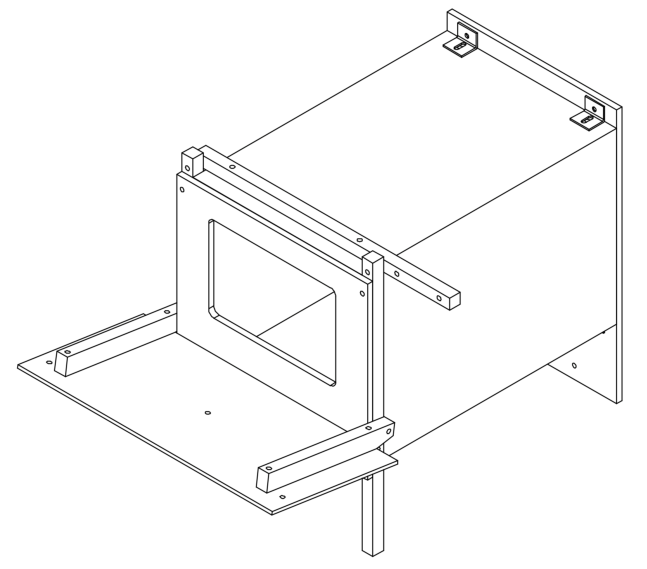
\includegraphics[width=0.2\textwidth]{Figures/aluminum-frame-concept.pdf}}%
 	}% end makebox
}% end title

\author{}
\date{}

\begin{document}

\maketitle

\section*{Features}
\addcontentsline{toc}{section}{Features}

\begin{flushleft}
	\begin{itemize}
		\fontsize{10}{12}\bfseries\selectfont
		\item Insulated aluminum frame with 6"x6"x10" interior chamber
		\item 400 Watt nichrome heating element with door safety switch
		\item 120 VAC power supply with surge and short protection
		\item Convection fan driven by bipolar motor
		\item Type K thermocouple for temperature feedback
		\item PIC16F883 microcontroller
		\item Convenient \mbox{7--segment} display and pushbutton user interface
	\end{itemize}
\end{flushleft}

\section*{Introduction}
\addcontentsline{toc}{section}{Introduction}

\emph{Easy--PCB} is a small, desktop convection oven for DIY reflow soldering at home.

As integrated circuits continue to become increasingly compact,
many $\mu$Controllers, FPGAs, and other ICs are no longer available in
DIP form for breadboard prototyping or iron soldering.
Similar to the shift away from PC parallel ports in the early 2000s,
the shift away from DIPs means modern electronics hobbyists need more
complicated equipment than their predessesors.

At the moment, hot air gun stations are sold commercially
and, very recently, several hackers have created open source designs
for IR solder ovens from converted toaster ovens.

\emph{Easy--PCB} is better than both because it combines the two;
a convection oven obviates the uneven heat absorbtion seen in infrared radiation based systems,
while controllable air flow prevents parts from being blown to never never PCB land.

\begin{center}
	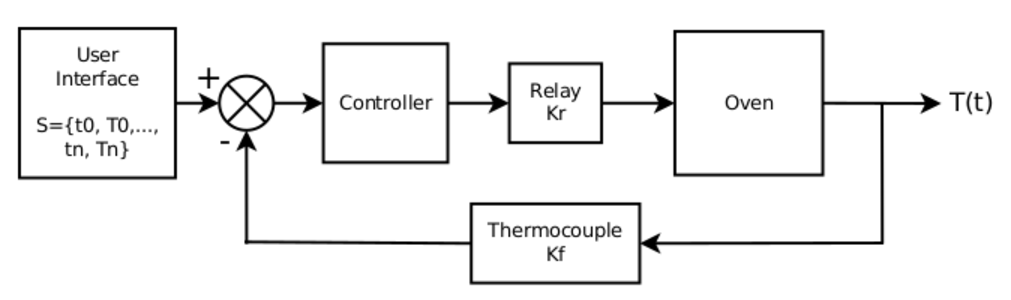
\includegraphics[width=\columnwidth]{Figures/control-system.pdf}
	\captionof{figure}{\emph{Easy--PCB} Control System}
	\label{control-system}
\end{center}

The temperature control system for \emph{Easy--PCB} is adverbaly adjective,
with only XX rise time and YY \% overshoot for a typical solder profile.
The use of temperature feedback and a reduction in dimensions from forced
convection are key to this success.

\begin{center}
	
\includegraphics[width=\columnwidth]{Figures/control-results.pdf}
	\captionof{figure}{Faithful Temperature Profile Control}
	\label{temperature-control-results}
\end{center}

In keeping with the hacker spirit, complete schematics, drawings,
source code, and materials lists for \mbox{\emph{Easy--PCB}} are appended to this datasheet.
All materials can be purchased online from Digi--Key, OSH Park and McMaster--Carr.com.
Design files are available on GitHub and were made exclusively from open source
or free software, including KiCad, DraftSight, NGSPICE, MPASM, and MPLAB IPE.
Finally, \emph{Easy--PCB} avoids any meta, ``chicken or the egg'' problems
because all its components can be soldered with an iron and clumsy hands.

\begin{figure*}
	\centering
	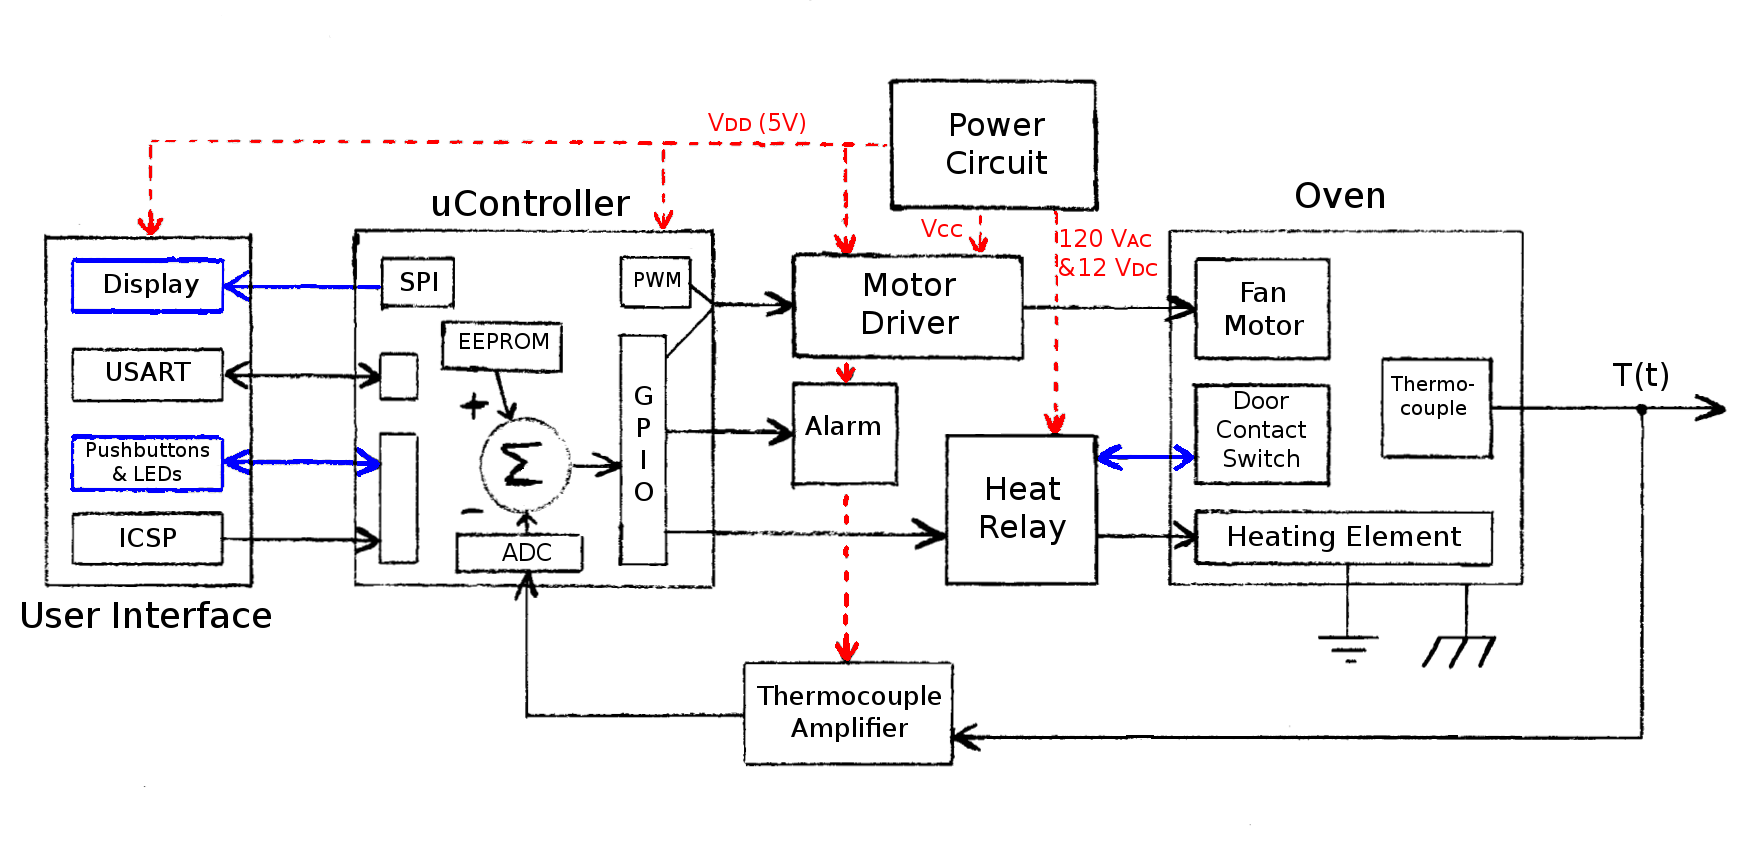
\includegraphics[width=\textwidth]{Figures/detailed-system-diagram.png}
	\caption{\emph{Easy--PCB} Detailed Control System}
	\label{detailed-system-diagram}
\end{figure*}

\pagebreak
\tableofcontents

\pagebreak
\section{User Interface}
\subsection{Its Easy as P--C--B!}

\emph{Easy--PCB} presents temperature and time information on a four digit LED display.
After pressing the green `start' button, the current temperature and process
runtime are alternately displayed every second.

\begin{center}
	\begin{minipage}[b]{0.45\columnwidth}
		\centering
		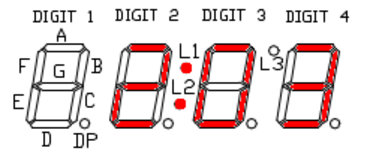
\includegraphics[width=\textwidth]{Figures/clock-display.pdf}
	\end{minipage}
	\begin{minipage}[b]{0.45\columnwidth}
		\centering
		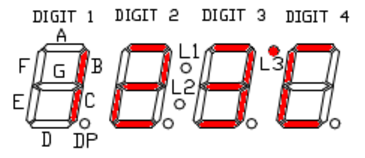
\includegraphics[width=\textwidth]{Figures/temperature-display.pdf}
	\end{minipage}
\end{center}

The red `stop' button can be pressed at anytime to quit the current process
or reset the microcontroller.

\begin{center}
	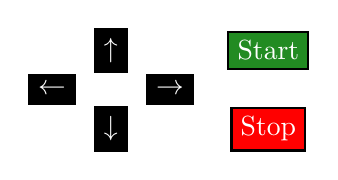
\begin{tikzpicture}[font=\fontsize{10pt}{11pt}\selectfont]
		\node [draw, thick,fill=black] (left) at (0cm, 0.5cm) {\textcolor{white}{$\leftarrow$}};
		\node [draw, thick,fill=black] (right) at (1.5cm, .5cm) {\textcolor{white}{$\rightarrow$}};
		\node [draw, thick, fill=black] (up) at (0.75cm, 1cm) {\textcolor{white}{$\uparrow$}};
		\node [draw, thick, fill=black] (down) at (0.75cm, 0cm) {\textcolor{white}{$\downarrow$}};
		\node [draw, thick, fill=ForestGreen] (start) at (2.75cm, 1cm) {\textcolor{white}{Start}};
		\node [draw, thick, fill=red] (stop) at (2.75cm, 0cm) {\textcolor{white}{Stop}};
	\end{tikzpicture}
	\captionof*{figure}{Pushbutton Interface}
\end{center}

Set point programming with the 4 nav keys is used to enter a time--temperature profile.
Use the `left' and `right' keys to move between set points and the `up' and `down'
keys to edit each set point value.

\begin{center}
	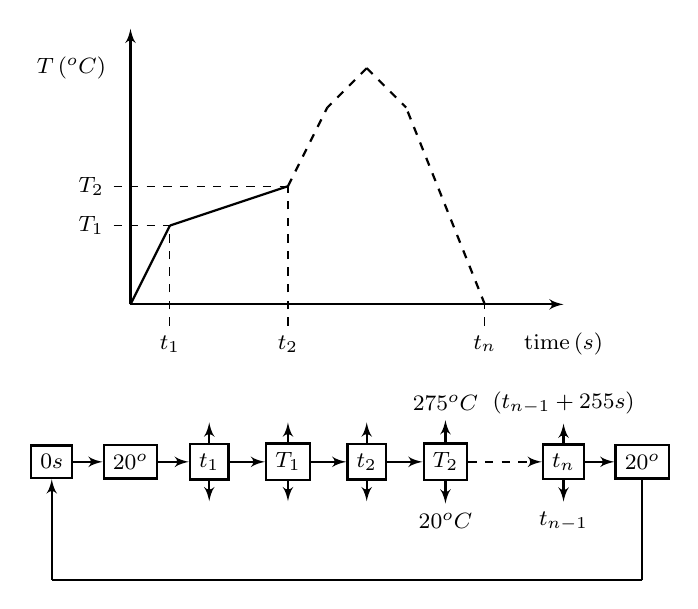
\begin{tikzpicture}[font=\fontsize{8pt}{9pt}\selectfont]
		\path [draw, -latex', thick] (1cm, 4cm) -- (1cm, 7.5cm);
		\path [draw, -latex', thick] (1cm, 4cm) -- (6.5cm, 4cm);
		\path [draw, thick] (1cm, 4cm) -- (1.5cm, 5cm);
		\path [draw, thick] (3cm, 5.5cm) -- (1.5cm, 5cm);
		\path [draw, thick, dashed] (3cm, 5.5cm) -- (3.5cm, 6.5cm);
		\path [draw, thick, dashed] (4cm,7cm) -- (3.5cm, 6.5cm);
		\path [draw, thick, dashed] (4cm,7cm) -- (4.5cm, 6.5cm);
		\path [draw, thick, dashed] (5.5cm,4cm) -- (4.5cm, 6.5cm);
		\node [draw, thick] (tzero) at (0cm, 2cm) {$0s$};
		\node [draw, thick] (Tzero) at (1cm, 2cm) {$20^{o}$};
		\path [draw, -latex', thick] (tzero) -- (Tzero);
		\node [draw, thick] (tone) at (2cm, 2cm) {$t_{1}$};
		\path [draw, -latex', thick] (Tzero) -- (tone);
		\node [draw, thick] (Tone) at (3cm, 2cm) {$T_{1}$};
		\path [draw, -latex', thick] (tone) -- (Tone);
		\node [draw, thick] (ttwo) at (4cm, 2cm) {$t_{2}$};
		\path [draw, -latex', thick] (Tone) -- (ttwo);
		\node [draw, thick] (Ttwo) at (5cm, 2cm) {$T_{2}$};
		\path [draw, -latex', thick] (ttwo) -- (Ttwo);
		\node [draw, thick] (tn) at (6.5cm, 2cm) {$t_{n}$};
		\path [draw, -latex', thick, dashed] (Ttwo) -- (tn);
		\node [draw, thick] (Tn) at (7.5cm, 2cm) {$20^{o}$};
		\path [draw, -latex', thick] (tn) to (Tn);
		\path [draw, thick] (Tn) -- (7.5cm, 0.5cm);
		\path [draw, thick] (7.5cm, 0.5cm) -- (0cm, 0.5cm);
		\path [draw, -latex', thick] (0cm,0.5cm) -- (tzero);
		\path [draw, -latex', thick] (tone) -- (2cm, 2.5cm);
		\path [draw, -latex', thick] (tone) -- (2cm, 1.5cm);
		\path [draw, -latex', thick] (Tone) -- (3cm, 2.5cm);
		\path [draw, -latex', thick] (Tone) -- (3cm, 1.5cm);
		\path [draw, -latex', thick] (ttwo) -- (4cm, 2.5cm);
		\path [draw, -latex', thick] (ttwo) -- (4cm, 1.5cm);
		\node (TtwoMax) at (5cm, 2.75cm) {$275^{o}C$};
		\node (TtwoMin) at (5cm, 1.25cm) {$20^{o}C$};
		\node (tnMax) at (6.5cm, 2.75cm) {$(t_{n-1}+255s)$};
		\node (tnMin) at (6.5cm, 1.25cm) {$t_{n-1}$};
		\path [draw, -latex', thick] (Ttwo) -- (TtwoMax);
		\path [draw, -latex', thick] (Ttwo) -- (TtwoMin);
		\path [draw, -latex', thick] (tn) -- (tnMax);
		\path [draw, -latex', thick] (tn) -- (tnMin);
		\node (t1label) at (1.5cm, 3.5cm) {$t_{1}$};
		\node (t2label) at (3cm, 3.5cm) {$t_{2}$};
		\node (tnlabel) at (5.5cm, 3.5cm) {$t_{n}$};
		\node (T1label) at (0.5cm, 5cm) {$T_{1}$};
		\node (T2label) at (0.5cm, 5.5cm) {$T_{2}$};
		\path [draw, dashed] (t1label) -- (1.5cm, 5cm);
		\path [draw, dashed] (t2label) -- (3cm, 5.5cm);
		\path [draw, dashed] (T1label) -- (1.5cm, 5cm);
		\path [draw, dashed] (T2label) -- (3cm, 5.5cm);
		\path [draw, dashed] (tnlabel) -- (5.5cm, 4cm);
		\node (Tlabel) at (0.25cm, 7cm) {$T\,(^{o}C)$};
		\node (tlabel) at (6.5cm, 3.5cm) {$\textrm{time}\,(s)$};
	\end{tikzpicture}
	\captionof*{figure}{Set Point Programming}
	\label{set-point-programming}
\end{center}

A total of 128 set points can be entered. The first set point is always $(0s,\,20^{o}C)$,
and the process will terminate at the next occurance of $20^{o}C$.
Temperatures can take any value in the range \mbox{$20\leq T \leq 275^{o}C$.}
The time between two points must be between \mbox{$0\leq t\leq255$ seconds.}

\section{Oven Design}

\subsection{Temperature Objectives}

\begin{figure*}
	\centering
	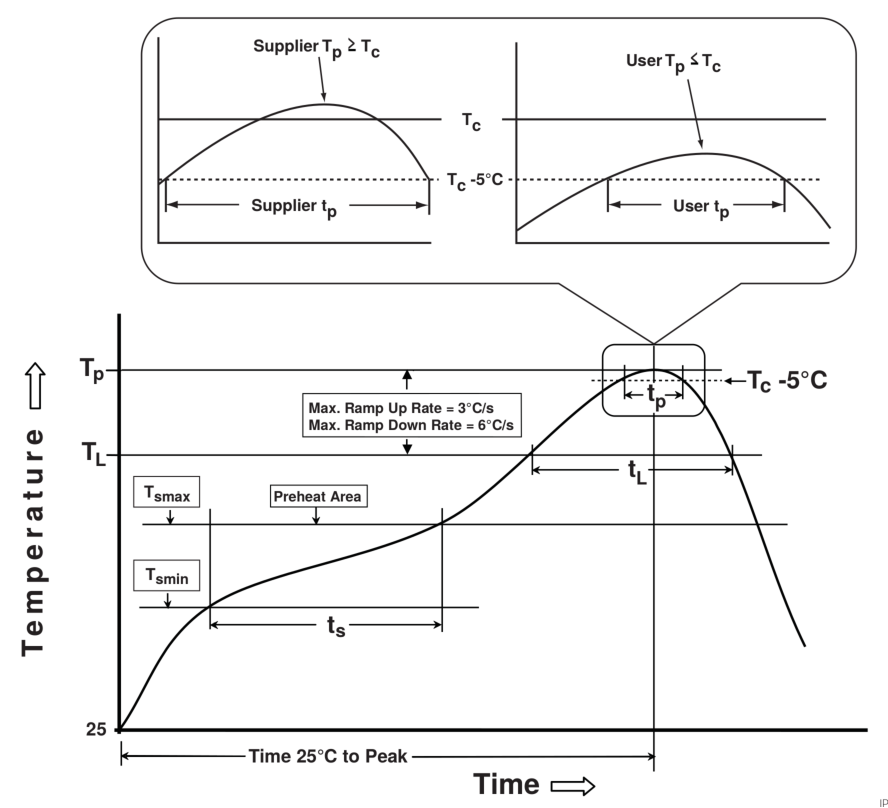
\includegraphics[width=0.7\textwidth]{Figures/standard-reflow-profile.pdf}
	\caption{Standard Solder Reflow Profile, per IPC/JEDEC STD-1-020D.1}
	\label{standard-reflow-profile}
\end{figure*}

A typical solder reflow profile is shown in
\hyperref[standard-reflow-profile]{\mbox{figure \ref{standard-reflow-profile}}}.
The optimal shape and peak temperature depend on the components and,
more significantly, on the use of leaded solder.
\begin{equation*}
T_{p}\approx T_{c}=\left\{\begin{array}{c c}
220-235^{o}C	&\textrm{Leaded solder}	\\
245-260^{o}C	&\textrm{Pb--free}	\\
\end{array}\right.
\end{equation*}
\begin{equation*}
t_{p}=\left\{\begin{array}{c c}
20s	&\textrm{Leaded solder}	\\
30s	&\textrm{Pb--free}	\\
\end{array}\right.
\end{equation*}

\emph{Easy--PCB} was designed from the ground up for faithfully producing these
reflow profiles. This design process for the thermodynamic system is detailed below.

\subsection{Thermodynamics Theory}

\textbf{Heat} is everyone's least favorite form of energy because it
tends to dissipate everywhere and is difficult to transform into useful work.
Nevertheless, it is a form of energy so it is measured in joules.
\begin{equation*}
Q:=\textrm{Heat}\,[\textrm{Joules}]
\end{equation*}

From a microscopic view, heat is the kinetic energy of gas molecules or the
vibrational energy of bonds in solids. In both cases, summed over every
molecule, every bond, and every vibrational mode in the system.

\begin{center}
	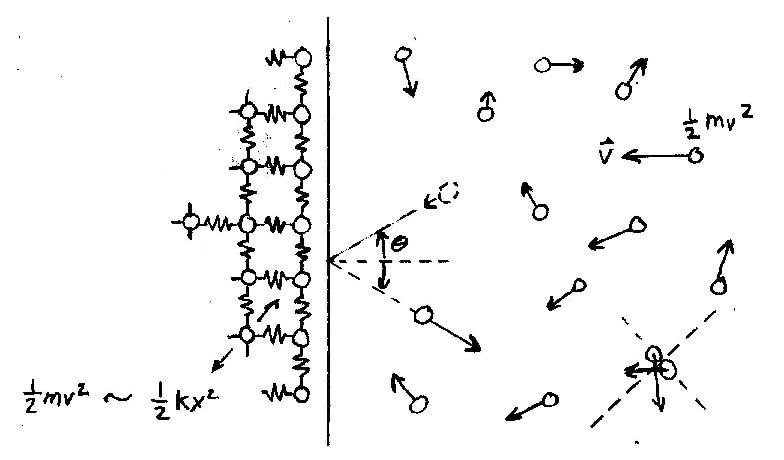
\includegraphics[width=1\columnwidth]{Figures/microscopic-view.pdf}
	\captionof{figure}{Heat Energy on a Molecular Scale}
	\label{microscopic-view}
\end{center}

\textbf{Temperature} is a potential field that measures an objects
tendancy to give up or absorb heat.
On average, heat always flows from regions of hotter temperature temperature
to lower temperature.
Temperature is usually measured in Kelvin or Celsius, which are related by
\begin{equation*}
T_{\textrm{Celsius}}=T_{\textrm{Kelvin}}+273.16.
\end{equation*}

Another way to think of temperature is a measure of heat density that also
incorporates the types of bonds (or lack thereof) in which heat energy is stored.
For example, a glacier contains more heat than a pot of boiling water, but
has a much lower heat density.

The relationship between temperature and heat stored in an object is given by
\begin{equation}
dQ=mc_{p}dT,
\label{specific-heat-eq}
\end{equation}
where $c_{p}$ is the specific heat of the material with units $\left[\frac{kJ}{kg*K}\right]$.

So heat flows spontaneously to reduce
temperature gradients, but how does heat flow and at what rate?
There are three mechanisms of heat transfer:
\emph{conduction}, \emph{convection}, and \emph{radiation}.

\textbf{Conduction} of heat is caused by molecular interactions,
such as the push--pull of nearby atomic bonds in solids or
elastic collisions between molecules of air.

The empirical relation for conduction is Fourier's Law, which
says the rate of heat transfer due to conduction is proportional
to both the difference in temperature and the media:
\begin{equation*}
\vec{q}=k\vec{\nabla}T
\end{equation*}
where $\vec{q}$ is the rate of heat transfer per unit surface area
and $k$ is the thermal conductivity of the medium with units
$\left[\frac{W}{m*K}\right]$.

In integral form, Fourier's Law is
\begin{equation*}
\frac{\delta Q}{\delta t}=k\oint_{S}\vec{\nabla}T*d\vec{A}.
\end{equation*}

And, in the one dimensional case,
\begin{equation}
\frac{\delta Q}{\delta t}=-kA\frac{\delta T}{\delta x}.
\label{1D-fouriers-law-eq}
\end{equation}

\textbf{Convection} is the second mechanism of heat transfer,
involving the bulk movement of particles driven by diffusion.

Every air molecule is moving in a random direction with random
kinetic energy, but a region of air with higher average kinetic
energy (temperature) will see more molecules leaving than entering
on average, because those leaving are moving faster than those
entering.

Note that in convection, no molecules gain or lose energy;
molecules of different energy simply trade places.

If a fan is used to apply work to a gas, the rate of convection
increases and then Newtons' Law of Cooling can predict the
rate of convection in gas near a solid surface of different
temperature.
\begin{equation}
\frac{dQ}{dt}=hA\Delta T
\label{newtons-cooling-law}
\end{equation}
where \(h\) is the heat transfer coefficient with \mbox{units \(\left[\frac{W}{m^{2}*K}\right]\)}.

\textbf{Radiation}, the third mechanism of heat transfer, is more
familiar to electrical engineers. In any material, electrons
have discrete amounts of energy based on the wave patterns that can
exist for the atomic geometry. When an electron spontaneously falls
to a less energetic patter, that energy is emitted as a photon of
light.

The classic, physics--history example is black body radiation,
when a metal is heated to high temperature and glows.
A more modern examle is the LED.

The empirical relation for radiation is the Stefan--Boltzmann Law,
which says that the total energy radiated, over all wavelengths
and per unit surface area, is proportional to the fourth power of
the body's temperature.
\begin{equation}
j^{*}=\sigma T^{4}
\end{equation}
where $\sigma$ is a proportionality constant derived from other
constants of nature.

\textbf{Mechanisms \& Media} Usually one mechanism of heat transfer
is dominant in a particular medium, so much so that we can ignore the
other two. Typically this means conduction in solids,
convection in fluids or gas, and radiation in space.
However, sometimes the picture is more complicated including
two cases in an oven:
\begin{enumerate}
	\item At the boundary of metal and air, where conduction
	and convection are both significant.
	\item In a thermocouple loop, where thermal diffusion (convection)
	of electrons is useful despite conduction still being dominant.
\end{enumerate}

\subsection{Thermodynamic Design}
\label{thermodynamic-design-section}

Most microwaves draw between 600 and 1200 Watts of power.
An IR toaster oven may draw 1500 Watts into its lamps.
How much power does \emph{Easy-PCB} need to produce the required temperature profiles?

Our approach for answering this question is to browse available parts on McMaster.com,
imagine how they would be assembled into an oven,
and then model their thermodynamic response using SPICE.

A first conceptual design of \emph{Easy--PCB} is shown in
\hyperref[first-oven-concept]{figure \ref{first-oven-concept}}.

\begin{center}
	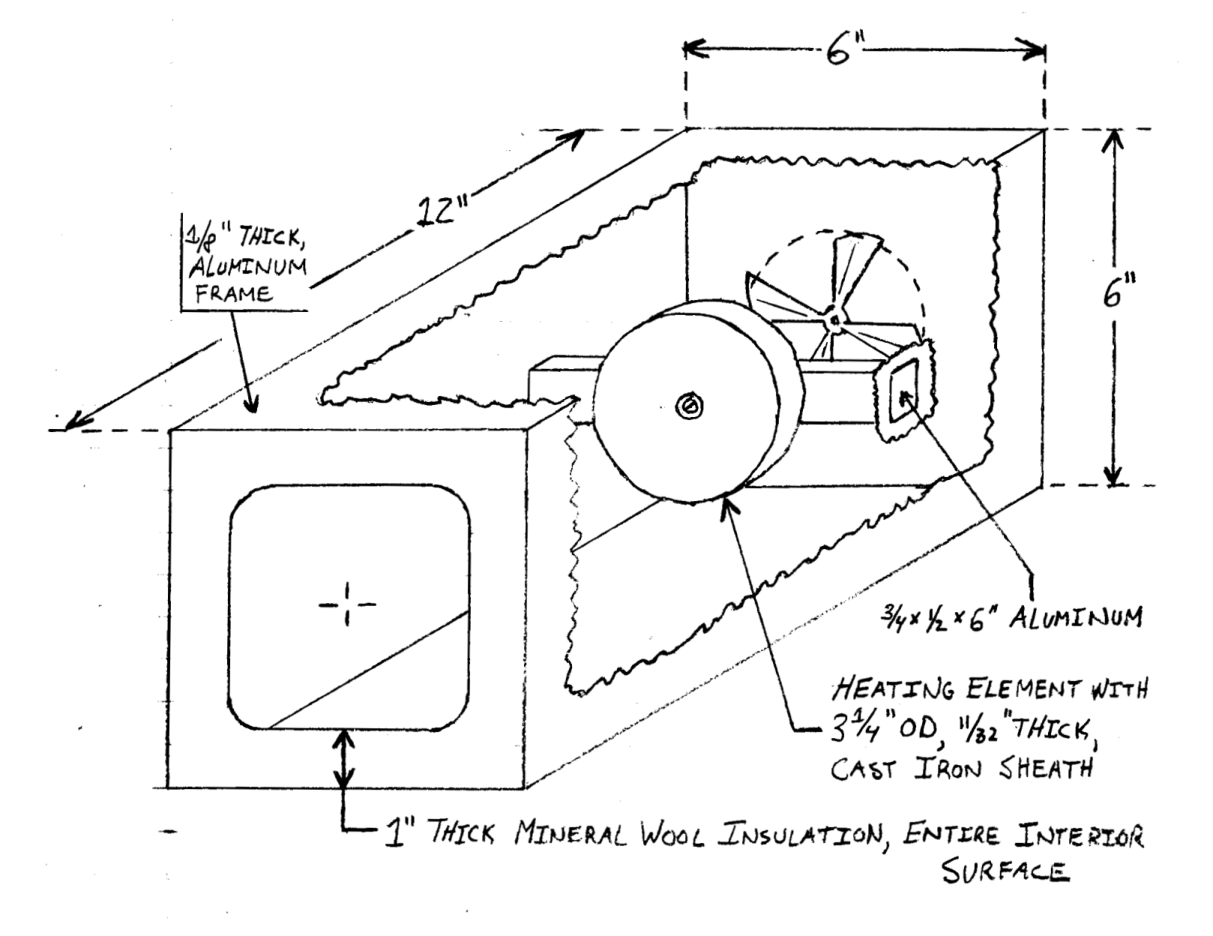
\includegraphics[width=\columnwidth]{Figures/first-oven-concept.pdf}
	\captionof{figure}{Concept for Thermodynamic System}
	\label{first-oven-concept}
\end{center}

\subsubsection*{Transmission through Metals \& Insulation}

In the concept, the oven chamber is isolated from the outside with walls of
mineral wool insulation and aluminum.
If the wall is relatively thin compared to the square root of its surface area,
then its heat transfer can be modeled as a 1--D transmission line, like shown in
\hyperref[unidirectional-conduction]{figure \ref{unidirectional-conduction}}.

\begin{center}
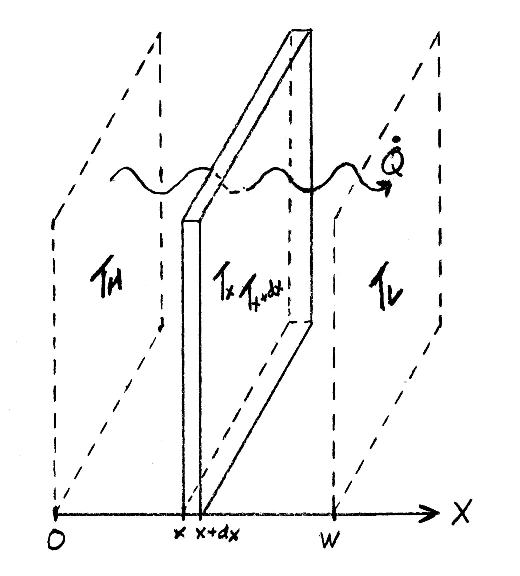
\includegraphics[width=0.85\columnwidth]{Figures/unidirectional-conduction.pdf}
\captionof{figure}{Heat Conduction in 1--D}
\label{unidirectional-conduction}
\end{center}

Assuming conduction is the dominant mechanism of heat transfer
and using Fourier's Law in 1--D,
(\hyperref[1D-fouriers-law-eq]{equation \ref{1D-fouriers-law-eq}})
the rate of heat passing through a thin slice is
\begin{equation*}
\frac{\delta Q}{\delta t}=-kA\frac{\delta T}{\delta x}
\end{equation*} 
 
And, from \hyperref[specific-heat-eq]{equation \ref{specific-heat-eq}},
the heat capacity of a thin slice of the metal sheath is
\begin{equation*}
dQ=(\rho A dx)c_{p}dT
\end{equation*}

Rewriting these equations to look like current-voltage relationships gives
\begin{equation}
\delta T=R_{x}\frac{\delta Q}{\delta t},
\quad R_{x}=\frac{\delta x}{kA}
\label{differential-resistance-eq}
\end{equation}
and
\begin{equation}
\frac{\delta Q}{\delta t}=C_{x}\frac{\delta T}{\delta t},
\quad C_{x}=\rho A c_{p} * \delta x
\label{differential-capacitance-eq}
\end{equation}

Values for thermal conductivity $k$, specific heat capacity $c_{p}$, and 
density $\rho$ of different materials are listed in
\hyperref[thermal-properties-table]{table \ref{thermal-properties-table}}.

Long metal bars and rods can also be modeled with equations
\ref{differential-resistance-eq} and \ref{differential-capacitance-eq}
if the heat loss along the length of the bar is assumed to be
negligible compared to heat transfered at the end faces.

\begin{center}
	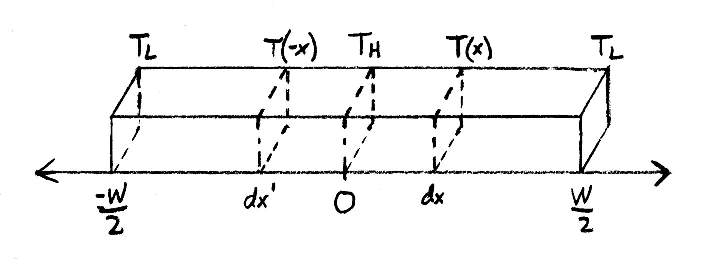
\includegraphics[width=1\columnwidth]{Figures/bidirectional-conduction.pdf}
	\captionof{figure}{1--D Conduction in Both Directions}
	\label{bidirectional-conduction}
\end{center}

For metal components where heat is injected at the center
of the part and dissipates symmetrically in either direction,
such as the support bar shown in
\hyperref[bidirectional-conduction]{figure \ref{bidirectional-conduction}}
or the metal sheath encasing the heating element,
the surface area can be doubled so that the transmission line
only needs to be integraded in the positive direction.
\begin{equation}
\left\{\begin{array}{c c c}
A_{x}	&\Rightarrow	&2A_{x}	\\
R_{x}	&\Rightarrow	&R_{x}/{2}	\\
C_{x}	&\Rightarrow	&2C_{x}	\\
\{x|-\frac{w}{2} \leq x \leq \frac{w}{2}\}	&\Rightarrow	&\{x|0 \leq x \leq \frac{w}{2}\}	\\
\end{array}\right.
\end{equation}

\begin{table*}
\centering
\caption{Thermal Conductivity, Specific Heat, and Density of Selected Materials}
\begin{tabular}{c | c | c | c | c}
\hline\hline
Material	&Linear Range $(^{o}C)$	&k \(\left(\frac{W}{m*K}\right)\)	&\(c_{p}\) \(\left(\frac{kJ}{kg*K}\right)\)	&\(\rho\) \((kg/m^{3})\)	\\
% Material	k	Cp	density	\\
\hline
Type 6061 Aluminum		&25	&167	&0.896	&2700	\\
Type 304 Stainless Steel	&0--100	&16.2	&0.5	&8000	\\
Cast Iron			&25	&55.0	&0.46	&6800--7800	\\
1.0 K--factor Insulation	&-	&0.1442	&-	&-	\\
0.23 K--factor Insulation	&-	&0.0332	&-	&-	\\
Nichrome NiCr C Alloy		&-	&0.450	&0.135	&8244	\\
Steatite L5 Ceramic		&-	&2.9	&0.92	&2710	\\
\hline\hline
\end{tabular}
\label{thermal-properties-table}
\end{table*}

\subsubsection*{Resistivity of Metal--Air Interface}

In the bulk volume of air, convection is the dominant form of heat
transfer and collisions are relatively rare. However, where the
air meets a solid surface, the net convection must go to zero because
there can be no net movement of air molecules into the solid.
Furthermore, every air molecule that reaches the surface experiences
a collision so there is 100\% conduction at the surface.

For some distance away from the surface, there is a larger than
normal chance of head--on collisions and slower rates of diffusion
due to the nearby wall. In this region, both conduction and convection
may be significant. To analyze this transition region,
we will start at the surface where there is 100\% conduction
because that is the mechanism we have equations for.

From the first law of thermodynamics, the rate of heat being stored
in a differential volume is equal to the rate of heat entering less
the rate of heat leaving the volume element.
\begin{equation*}
\frac{\delta Q_{\textrm{stored}}}{\delta t}=
\frac{\delta Q_{\textrm{in}}}{\delta t}-
\frac{\delta Q_{\textrm{out}}}{\delta t}
\end{equation*}

Looking back at
\hyperref[unidirectional-conduction]{figure \ref{unidirectional-conduction}},
the differential volume element is a plane, so
\begin{equation*}
\frac{\delta Q_{\textrm{stored}}}{\delta t}=
\frac{\delta Q_{x}}{\delta t}-
\frac{\delta Q_{x+\delta x}}{\delta t}.
\end{equation*}

Substituting in
\hyperref[heat-capacity-eq]{equation \ref{specific-heat-eq}}
for stored heat capacity and
\hyperref[1D-fouriers-law-eq]{equation \ref{1D-fouriers-law-eq}} for
conduction through the element yields a transport equation.

\begin{equation}
mc_{p}\frac{\delta T}{\delta t}=kA\frac{\delta T}{\delta x}
\label{transport-eq}
\end{equation}

This cannot be solved analytically unless space and time are independent.
Sorry Albert.
\begin{equation}
T(x\,,t)=T_{x}(x)*T_{t}(t)
\end{equation}

Applying the chain rule to equation \ref{transport-eq}
\begin{equation*}
mc_{p}\frac{\delta T_{t}(t)}{\delta t}T_{x}(x)=
kA\frac{\delta T_{x}(x)}{\delta x}T_{t}(t)
\end{equation*}
and separating variables gives
\begin{equation*}
mc_{p}\frac{\delta T_{t}(t)}{\delta t}*\frac{1}{T_{t}(t)}=
kA\frac{\delta T_{x}(x)}{\delta x}*\frac{1}{T_{x}(x)}.
\end{equation*}

The only way for the equality to be true for all space and time
is if both sides are equal to a common constant.
\begin{equation*}
\alpha=mc_{p}\frac{\delta T_{t}(t)}{\delta t}*\frac{1}{T_{t}(t)}
\end{equation*}
\begin{equation*}
\alpha=kA\frac{\delta T_{x}(x)}{\delta x}*\frac{1}{T_{x}(x)}
\end{equation*}

Each of these can be solved by separation of variables.
\begin{equation*}
\frac{\alpha}{kA}\delta x=\frac{\delta T_{x}(x)}{T_{x}(x)}
\end{equation*}

\begin{equation*}
\frac{\alpha}{kA}\int \delta x=\int \frac{1}{T_{x}(x)}*\delta T_{x}(x)
\end{equation*}

\begin{equation*}
\frac{\alpha x}{kA}=ln\left(T_{x}(x)\right)+\beta_{1}
\end{equation*}

\begin{equation*}
T_{x}(x)=\beta_{1}^{'}e^{\nicefrac{\alpha x}{kA}}
\end{equation*}

Similarly for time,
\begin{equation*}
T_{t}(t)=\beta_{2}^{'}e^{\nicefrac{\alpha t}{mc_{p}}}.
\end{equation*}

Recombining the independent components gives
\begin{equation*}
\Delta T(x\,,t)=\beta_{1}^{'}\beta_{2}^{'}e^{\nicefrac{\alpha x}{kA}+\nicefrac{\alpha t}{mc_{p}}}
\end{equation*}

The boundary conditions are that at $t=0$ and $x=0$, the temperature difference is
the initial temperature difference, and at $t\rightarrow\infty$ and $x\rightarrow\infty$,
the temperature difference dissipates to zero.
\begin{equation*}
\Delta T(x\,,t)=\Delta T_{0}e^{\nicefrac{-\alpha x}{kA}-\nicefrac{\alpha t}{mc_{p}}}
\end{equation*}

Now, for the sake of physical intuition we can write
\begin{equation}
\Delta T(x\,,t)=\Delta T_{0}e^{-(\nicefrac{x}{\delta}+\nicefrac{t}{\tau})},
\label{transport-solution-eq}
\end{equation}
where $\delta$ is a `skin depth' over which the spacial gradient decays to $1/e$ its
initial value and $\tau$ is a time constant related to the skin depth by
\begin{equation}
\tau=\frac{mc_{p}}{kA}\delta.
\label{transport-time-constant-eq}
\end{equation}

Make some arguments and plot the temperature and heat transfer curves.
Assume steady state and somehow that active cooling makes it all valid.

Applying Fourier's law to the temperature profile found in
\hyperref[transport-solution-eq]{equation \ref{transport-solution-eq}},
gives us the rate of heat trasfer in the air due to conduction.
\begin{equation*}
\frac{dQ}{dt}=-kA\frac{dT}{dx}=
\frac{kA}{\delta}\Delta T_{0}e^{-(\nicefrac{x}{\delta}+\nicefrac{t}{\tau})}
\end{equation*}

Again assuming steady state, the rate of heat trasfer at any distance from
the wall is equal to the rate of conduction at the wall.
\begin{equation}
\frac{dQ}{dt}=\frac{kA}{\delta}\Delta T_{0}=h_{c}A\Delta T_{0}
\label{derived-cooling-law-eq}
\end{equation}

This is the information we were after and, ironically, it turns out this is 
Newton's Law of Cooling
(\hyperref[newtons-cooling-law]{equation \ref{newtons-cooling-law}})
where $h_{c}=\nicefrac{k}{\delta}$. Since we do not have any way of predicting
the skin depth except by experimentation, some common values for
the convective heat transfer coefficient $h_{c}$ are listed in
\hyperref[typical-h-values-table]{table \ref{typical-h-values-table}}.

\begin{table}
	\centering
	\caption{Typical Convective Heat Transfer Coefficients}
	\begin{tabular}{c | c | c}
	\hline\hline
	Fluid	&Conv.	&$h_{c}\,\left[\frac{W}{m^{2}*K}\right]$	\\
	\hline
	Gases, \& dry vapors	&free	&$0.5-1000$	\\
				&forced	&$10-1000$	\\
	Water \& liquids	&free	&$50-3000$	\\
				&forced	&$50-10000$	\\
	Boiling Water		&-	&$3-100$	\\
	Condensing $H_{2}O$ Vapor&-	&$5-100$	\\
	\hline\hline
	\end{tabular}
	\label{typical-h-values-table}
\end{table}

\hyperref[derived-cooling-law-eq]{Equation \ref{derived-cooling-law-eq}}
can be rewrittent to look like Ohms' law for SPICE analysis.
\begin{equation}
\Delta T=R_{c}\frac{dQ}{dt},\quad R_{c}=\frac{1}{h_{c}A}=\frac{\delta}{kA}
\label{cooling-resistance-eq}
\end{equation}

\subsubsection*{Heat Capacity of Chamber Air}

The heat capacity of the air in the chamber cannot be analyzed
with constant coefficient assumptions.
\begin{equation}
dQ=m(T)c_{p}(T)dT
\label{specific-heat-with-variable-coefficients-eq}
\end{equation}

\begin{table}
	\centering
	\caption{Thermal Properties of Air}
	\begin{tabular}{c | c | c | c}
\hline\hline
$T\,[^{o}C]$	&$\rho\left[\frac{kg}{m^{3}}\right]$	&$c_{p}\left[\frac{kJ}{kg*K}\right]$	&$k\left[\frac{W}{m*K}\right]$	\\
\hline
20	&1.205	&1.005	&0.0257	\\
40	&1.127	&1.005	&0.0271	\\
60	&1.067	&1.009	&0.0285	\\
80	&1.000	&1.009	&0.0299	\\
100	&0.946	&1.009	&0.0314	\\
120	&0.898	&1.013	&0.0328	\\
140	&0.854	&1.013	&0.0343	\\
160	&0.815	&1.017	&0.0358	\\
180	&0.779	&1.022	&0.0372	\\
200	&0.746	&1.026	&0.0386	\\
250	&0.675	&1.034	&0.0421	\\
300	&0.616	&1.047	&0.0454	\\
\hline\hline
	\end{tabular}
	\label{air-properties-table}
\end{table}

From \hyperref[air-properties-table]{table \ref{air-properties-table}},
we can see that the specific heat of air does not vary much over the
temperature range of the oven; less than 0.3\% from $c_{p(20^{o}C)}$
over the range $20-300^{o}C$. However, the density and mass of air
in the chamber may change significantly.

Assuming that the air in the chamber behaves like an ideal gas
and is made up of the normal percentages of $N_{2}$, $O_{2}$, $CO_{2}$, etc., then mass and temperature are related by
\begin{equation*}
PV=\frac{m}{M}RT\quad\Rightarrow\quad m(T)=\frac{MPV}{R}T
\end{equation*}
where the ideal gas constant is
\begin{equation*}
R=5.00745\,\left[\frac{\textrm{atm}*\textrm{in}^{3}}{\textrm{mol}*K}\right]
\end{equation*}
and the molar mass of air is
\begin{equation*}
M=28.97\,\left[\frac{g}{\textrm{mol}}\right]
\end{equation*}

For the first oven concept in
\hyperref[first-oven-concept]{figure \ref{first-oven-concept}},
the volume of the chamber is fixed in natural units of $in^{3}$
and there are likely small leaks that let the chamber
pressure equilibrate to atmospheric pressure $1\,\textrm{atm}$.

Substituting $m(T)$ into
\hyperref[specific-heat-with-variable-coefficients-eq]
{equation \ref{specific-heat-with-variable-coefficients-eq}},
converting from absolute Kelvin scale to Celsius, and
manipulating to look like a current--voltage relationship results in
\begin{equation}
\frac{dQ}{dt}=C_{c}(T)\frac{dT}{dt}
\end{equation}
where
\begin{equation}
C_{c}(T)=\frac{c_{p(20^{o}C)}MPV}{R(T+273.16^{o}C)}.
\label{bulk-air-capacitance-eq}
\end{equation}

Equivalently,
\begin{equation*}
C_{c}(T)=\frac{\left(5.8143\left[\frac{J}{in^{3}}\right]\right)*V}{T+273.16^{o}C}.
\end{equation*}

\subsubsection*{Variable Capacitor for Chamber Air}

Unfortunately, SPICE does not have a primitive circuit element for
a variable capacitor.
Before simulating and iterating the oven design, we must build a
SPICE subcircuit to model heat capacity of ideal gasses.
The subcircuit black box must have two terminals with I--V relation
\begin{equation*}
i_{c}=C(v_{c})\frac{dv_{c}}{dt},
\label{capacitor-iv-relation}
\end{equation*}
or, alternatively,
\begin{equation}
\int i_{c}dt=\int C(v_{c})dv_{c}.
\label{capacitor-integrated-iv-relation}
\end{equation}

The left side of \hyperref[capacitor-integrated-iv-relation]
{equation \ref{capacitor-integrated-iv-relation}} is an integrator,
which can be implemented with a buffer and a capacitor.
For the SPICE circuit shown in
\hyperref[variable-capacitance-circuit]{figure \ref{variable-capacitance-circuit}},
the integrated current is proportional to the voltage of
the `int' node.
\begin{equation*}
\int i_{c}dt=C_{\textrm{int}}*v_{int}
\end{equation*}

\begin{center}
	\includegraphics[width=0.75\columnwidth]{Figures/variable-capacitance-circuit.pdf}
	\captionof{figure}{Voltage Variable Capacitor in SPICE}
	\label{variable-capacitance-circuit}
\end{center}

For the right side of
\hyperref[capacitor-integrated-iv-relation]
{equation \ref{capacitor-integrated-iv-relation}},
it can be solved for the variable heat capacitance
of an ideal gas found in
\hyperref[bulk-air-capacitance-eq]{equation \ref{bulk-air-capacitance-eq}}.
\begin{equation*}
\begin{array}{c l}
\int C(v_{c})dv_{c}	&=\frac{c_{p}MPV}{R}\int\frac{dv_{c}}{v_{c}+273.16}	\\
&\\
&=\frac{c_{p}MPV}{R}ln(v_{c}+273.16)+A	\\
\end{array}
\end{equation*}

Recombining the left and right halves gives
\begin{equation*}
C_{int}v_{int}=\frac{c_{p}MPV}{R}ln(v_{c}+273.16)+A,
\end{equation*}
which can be solved to find a nonlinear expression
for a dependent source $v_{c}$.

Solving...
\begin{equation*}
\frac{RC_{int}}{c_{p}MPV}*v_{int}=ln(v_{c}+273.16)+A
\end{equation*}

\begin{equation*}
v_{c}=A^{'}e^{\nicefrac{v_{int}}{B}}-273.16
\end{equation*}

Finally, applying boundary conditions $v_{c}(0)=0$ and $v_{int}(0)=0$ gives
\begin{equation}
v_{c}=273.16\left(e^{\nicefrac{v_{int}}{B}}-1\right)
\end{equation}
where constant $B$ is
\begin{equation}
\begin{array}{c c l}
B&=&\frac{c_{p}MP}{R}*V*C_{int}\\
&&\\
&=&\left(5.8413\left[\frac{J}{in^{3}}\right]\right)*V*C_{int}\\
\end{array}
\end{equation}
and $V$ is the constant volume of air.

\begin{table}
	\centering
	\caption{Nichrome Wire Properties (NiCr C)}
	\begin{adjustbox}{max width=\columnwidth}
	\begin{tabular}{c | c c c c}
\hline
Composition	&59.2\%Ni	&16\%Cr	&23.5\%Fe	&1.3\%Si	\\
Resistivity ($\rho$)	&$675*\pi$	&$\left[\frac{\Omega*\textrm{mil}^{2}}{ft}\right]$	&$1.12$	&$[\mu \Omega*m]$	\\
Melting Pt.	&1350	&$[^{o}C]$	&	&	\\
\hline\hline
Temp. [$^{o}C$]	&20	&93	&204	&315	\\
\% $\rho$ Increase	&0	&1.7	&3.5	&5.2	\\
\hline
	\end{tabular}
	\end{adjustbox}
	\label{nichrome-properties-table}
\end{table}

\subsection{Design Iteration \& SPICE Modeling}

Many designs with different shapes, sizes, metals, insulators,
heating elements, and wattage levels were modeled in SPICE for their
thermodynamic response to a unit step signal from the power relay.
The primary parameter of interest was the heating rate of the air
in the chamber.

The SPICE models were based on the equations from
\hyperref[thermodynamic-design-section]{section \ref{thermodynamic-design-section}};
material properties from tables \ref{thermal-properties-table}, \ref{typical-h-values-table},
\ref{air-properties-table}, and \ref{nichrome-properties-table}; and
geometry of the design.
Unitwise, $1\,\textrm{Volt}=1^{o}C$, $1\,\textrm{Ampere}=1\,\textrm{Watt}$,
\mbox{and $1\,\textrm{Coulomb}=1\,\textrm{Joule}$.}

Eventually a design using 135 ft of 51 mil nichrome wire inside a 8"x8"x12"
aluminum frame was selected.

The shape of the aluminum frame is shown in
\mbox{\hyperref[aluminum-frame-concept]{figure \ref{aluminum-frame-concept}}}.
The inside of the frame is lined with 1" thick mineral wool insulation,
leaving an inside chamber with dimensions 6"x6"x10".
A fan is mounted in the back.

\begin{figure}
	\centering
	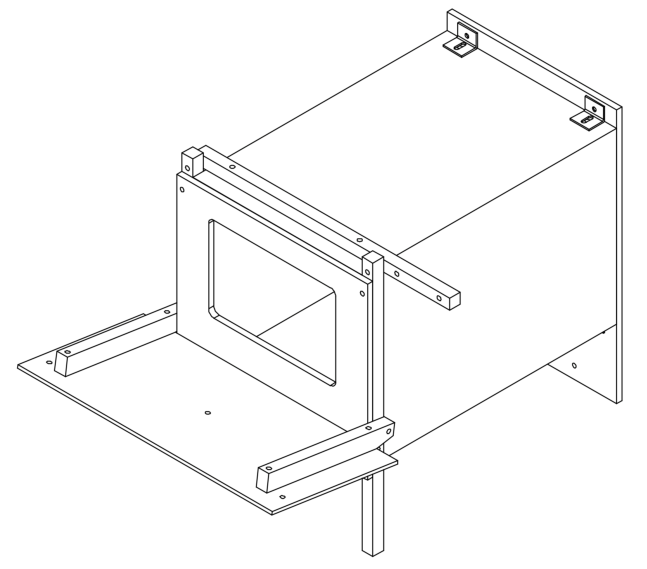
\includegraphics[width=\columnwidth]{Figures/aluminum-frame-concept.pdf}
	\caption{Aluminum Frame Concept}
	\label{aluminum-frame-concept}
\end{figure}

Inside the frame, nichrome wire is mounted using high temperature
ceramic spacers for electrical insulation. Structurally, the nichrome
element is tensioned by two size 10 steel bolts spanning the width of the
chamber, as shown in
\mbox{\hyperref[heating-element-concept]{figure \ref{heating-element-concept}}}.
Direct contact between the nichrome heating element and the chamber air
is critical for fast heating rates.

\begin{figure}
	\centering
	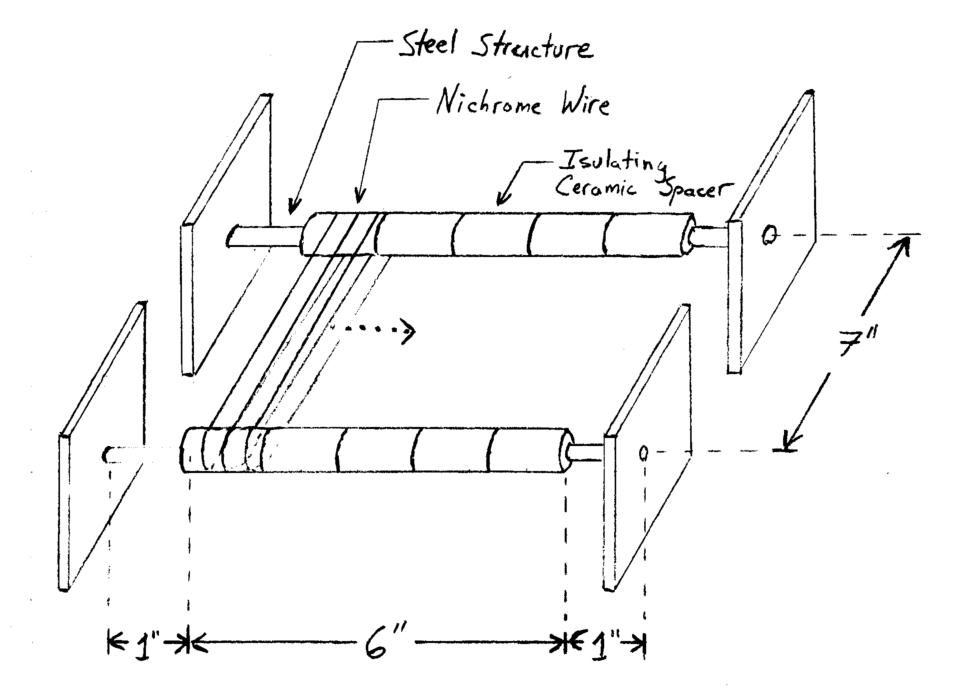
\includegraphics[width=\columnwidth]{Figures/heating-element-concept.pdf}
	\caption{Heating Element Concept}
	\label{heating-element-concept}
\end{figure}

The thermodynamic model is shown in
\hyperref[thermodynamic-spice-circuit]{figure \ref{thermodynamic-spice-circuit}}.

The electrical resistance of the nichrome wire is given by
\begin{equation*}
R_{\textrm{electric}}=675\left[\frac{ft}{mil^{2}}\right]*
\frac{l}{OD^{2}}
\end{equation*}
where $l$ is the wire length in feet and $OD$ is the wire diameter in mils (0.001").

DISCUSSION/MATH OF MODEL VALUES

\begin{figure*}
	\centering
	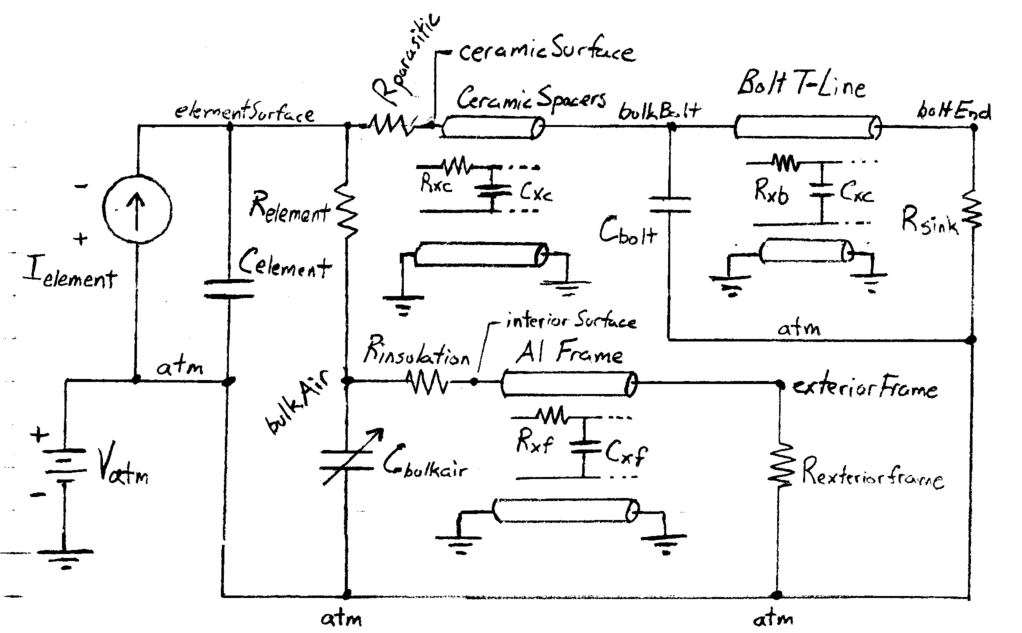
\includegraphics[width=0.8\textwidth]{Figures/thermodynamic-spice-circuit.pdf}
	\caption{Thermodynamic SPICE Model Circuit Diagram}
	\label{thermodynamic-spice-circuit}
\end{figure*}

The circuit netlist passed to SPICE is listed in
\hyperref[heat-model-listing]{section \ref{heat-model-listing}}.
The circuit was modeled for its transient reponse if the heating element
were connected to 120 VAC power for 100 second.
The results are shown in
\hyperref[heat-model-results]{figure \ref{heat-model-results}}.

\begin{figure}
	\centering
	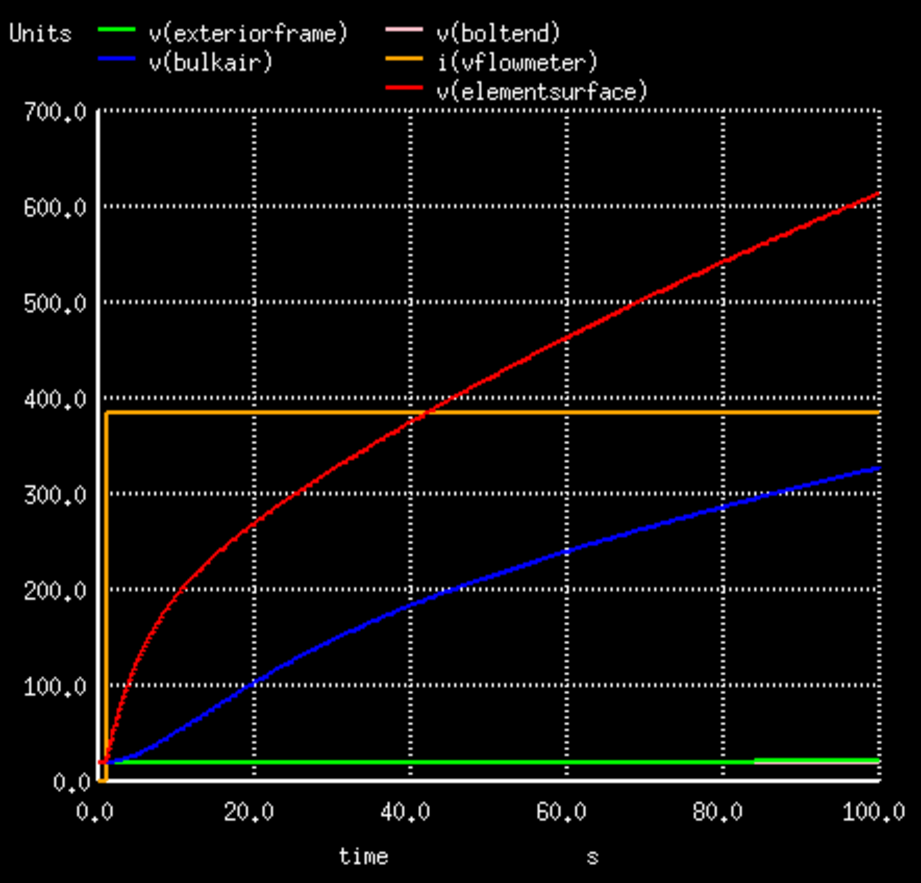
\includegraphics[width=1\columnwidth]{Figures/heat-model-results.pdf}
	\caption{Simulated Temperature Response to a Unit Step}
	\label{heat-model-results}
\end{figure}

\section{User Interface Design}

\subsection{Separate, Front--Facing PCB}

The user interface is designed to be assembled on a separate PCB
from the main controller board. The separation allows the high power
components and power entry points to be mounted on the back of the
oven---far away from the user.
The user interface PCB is mounted near the door and has no
voltages greater than 5 V for safety. Everything on the front PCB
is shown in blue in \emph{Easy--PCB} block diagram
\mbox{(\hyperref[detailed-system-diagram]{figure \ref{detailed-system-diagram}})}.

\begin{center}
	\includegraphics[width=0.75\columnwidth]{Figures/front-PCB-image.pdf}
	\captionof*{figure}{Front--Facing PCB}
	\label{front-facing-pcb}
\end{center}

The front PCB was designed with mounting points
such that a contact switch mates with the oven door and 
level pushbutton heights for an enlosure or facade.

The user interface board contains a 4--digit, 7--segment, common--cathode
display and a matching common--cathode driver. The display driver
is connected to the controller board via 4 wire serial peripheral interface (SPI).
From the MAX7219 datasheet, the worst case current draw by the display driver
is
\begin{equation}
I_{\textrm{LED Display}}<200\,mA.
\end{equation}

There are 6 active low
pushbuttons on the front--facing board that are designed to be used
with the internal pull--up resistors available in \textrm{PORTB}
on the PIC microcontroller. The pushbutton circuit is shown in
\hyperref[pushbutton-circuit]{figure \ref{pushbutton-circuit}}.

\begin{figure}
	\centering
	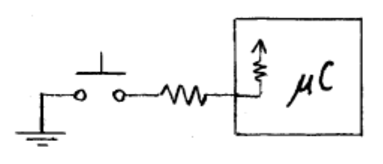
\includegraphics[width=0.6\columnwidth]{Figures/pushbutton-circuit.pdf}
	\caption{Pushbutton Circuit using Interal Pull--Ups}
	\label{pushbutton-circuit}
\end{figure}

The two active--high LEDs that are built into the red and green pushbuttons
need current limiting resistors to protect both the diode and the $\mu$Controller.
The LEDs in the RP3508 pushbuttons are rated for forward current of 20 mA and 1.8 V.
For ten milliamp intensity,
\begin{equation*}
R_{\textrm{limit}}=\frac{V_{DD}-V_{fwd}}{I_{fwd}}=\frac{5-1.8\,V}{10\,mA}=320\,\Omega
\end{equation*}

\subsection{Alarm, ICSP, and USART}

This section is loaded with assumption and implication.

First, if you look at the block diagram in
\mbox{\hyperref[detailed-system-diagram]{figure \ref{detailed-system-diagram}}},
the alarm is supposed to actuate the oven door for the control system.
The only way to make this true is to design a horribly annoying alarm
and not acknowledge it is a part of the user interface.

The audio alarm is provided by a 2 kHz piezoelectric element and a small BJT
amplifier circuit, like shown in
\hyperref[piezo-circuit]{figure \ref{piezo-circuit}}.

\begin{figure}
	\centering
	\includegraphics[width=0.7\columnwidth]{Figures/piezo-circuit.pdf}
	\caption{Piezo Alarm}
	\label{piezo-circuit}
\end{figure}

Second, the PIC In--Circuit Serial Programming (ICSP) header is a part of the user
interface more than it is a part of the controller because I doubt \emph{Easy--PCB}
will ever be bug free and I am judging my audience to be other hackers.

The ICSP circuit is shown in
\hyperref[pic16f883-circuit]{figure \ref{pic16f883-circuit}}.
The low voltage programming is geared toward production environments
or products which may need firmare updated by other ICs in the system.
It is not necessary for programming with the PICkit3 at home.
The data and clock (DAT and CLK) pins can shared with other hardware
as long as there is no bus contention during programming.

Third, a header for USART is provided for debugging
\ldots another assumption being made about my audience.

\subsection{Safety Stop Button}

INTERUPT ROUTINE ON STATE DIAGRAM?

\section{Thermocouple Amplifier Design}

\subsection{Thermocouple Theory}

To develop accurate temperature control, real time temperature feedback
is necessary. The temperature is too hot for thermisters or temperature ICs,
so old school thermocouples must be used.

The Seebeck voltage is the electromotive force that develops due to temperature
gradient in a conductive loop made of two different metals. It is described by
\begin{equation}
E_{S}=\int _{TR}^{T}\alpha_{A,B}dT,
\end{equation}
where $T$ and $T_{R}$ are the temperatures of the hot and cold junctions and
$\alpha_{A,B}$ is the Seebeck coefficient between metals $A$ and $B$.

A type--K thermocouple was selected because they are readily available and
resist oxidation at temperatures up to $1260^{o}C$.
From the ``Manual on the use of Thermocouples in Temperature Measurement'' \mbox{(STP 470A)}, the nominal
Seebeck coefficients for type--K and J thermocouples are
\begin{equation}
\alpha_{KP,KN}=\left\{\begin{array}{c c}
0^{o}C		&39.4\,\mu V/^{o}C	\\
200^{o}C	&40.0\,\mu V/^{o}C	\\
400^{o}C	&42.3\,\mu V/^{o}C	\\
\end{array}\right.,
\end{equation}
and
\begin{equation}
\alpha_{JP,JN}=\left\{\begin{array}{c c}
0^{o}C		&50.2\,\mu V/^{o}C	\\
200^{o}C	&55.8\,\mu V/^{o}C	\\
400^{o}C	&55.3\,\mu V/^{o}C	\\
\end{array}\right..
\end{equation}

The positive wire $KP$ is one of the following alloys: Chromel, Tophel, T--1, or ThermoKanthal KP.
The negative wire $KN$ is Alumel, Nial, T--2, or ThermoKanthal KN.

\subsection{Amplifier Design}

\begin{figure}
	\centering
	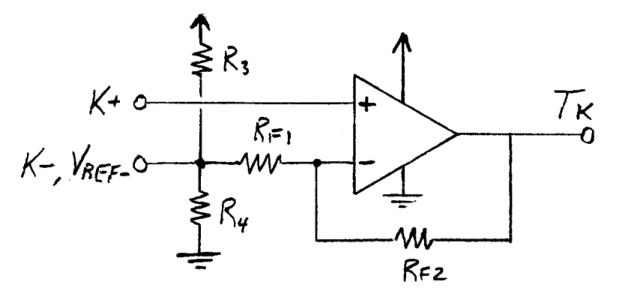
\includegraphics[width=\columnwidth]{Figures/thermocouple-amplifier.pdf}
	\caption{Thermocouple Amplifier Circuit}
	\label{thermocouple-amplifier}
\end{figure}

The thermoelectric potential in a K loop is very small; 
for a temperature difference of $T-T_{R}=255^{o}C$,
the voltage developed is only on the order of $E_{S}=10.2\,mV$.
Consequently, the signal needs to be amplified before it can be read by an ADC.

The op amp circuit shown in
\hyperref[thermocouple-amplifier]{figure \ref{thermocouple-amplifier}}
can be used. A two resistor voltage dividor network is used to lift the reference
voltage above 0 V, because only 0 and 5 V power rails are available and most
op amps cannot swing their output the full range of the supply rails.

The \textrm{PIC16F883}'s ADC has the ability to operate between $V_{SS}$ and $V_{DD}$ (0 and 5 V),
but external reference voltages can also be used. Therefore, we should pass the
negative voltage reference for the op amp into the negative voltage reference pin of the PIC,
and then design the amplifier gain such that the maximum temperature range of $0\leftrightarrow255\,^{o}C$
is mapped linearly to $V_{ref-}\leftrightarrow5\,V$

\begin{equation*}
	\frac{R_{f2}}{R_{f1}}=
	\frac{V_{\textrm{ADC(max)}}}{V_{\textrm{K(max)}}}=
	\frac{3.3\,V}{10.2\,mV}
\end{equation*}
\begin{equation}
\textrm{type--K:}\quad R_{f2}=323.5*R_{f1}
\end{equation}

Similarly, if a type--J thermocouples is used, the resistor ratio should be
\begin{equation}
\textrm{type--J:}\quad R_{f2}=233.2*R_{f1}
\end{equation}

\subsection{Thermistor Amplifier Design}

\section{Motor Driver Design}

\subsection{Bipolar Motor Selection}

The combination of needing motors and relays and already being plugged in to a 
120 VAC source led to the decision to create a 12 V power rail. The 12 V rail
will only be used by components that are not particularly affected by a noisy
signal, so this rail does not need active regulation.

With a 12 V rail in mind, there are many more choices for motors to drive the fan.
A bipolar stepper motor was chosen because of its open speed control in low torque applications.

\begin{center}
	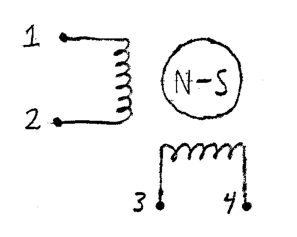
\includegraphics[width=0.2\textwidth]{Figures/bipolar-motor.pdf}
	\captionof{figure}{Bipolar Stepper Motor}
\end{center}

The 44M100D2B motor by Portescap rotates $3.6^{o}$ per change in polarity--i.e. 100 step increments,
according to the polarities in
\hyperref[44M100D2B-polarities]{table \ref{44M100D2B-polarities}}.

\begin{table}
\centering
\caption{Step Polarites for 44M100D2B Motor}
\begin{tabular}{c | c | c | c | c | c}
\hline\hline
CW	&Step	&Red (1)&Gry (2)&Yel (3)&Blk (4)	\\
\hline\hline
\verb1|1	&1	&+	&-	&+	&-	\\
\verb1|1	&2	&+	&-	&-	&+	\\
\verb1|1	&3	&-	&+	&-	&+	\\
v		&4	&-	&+	&+	&-	\\
\hline\hline
\end{tabular}
\label{44M100D2B-polarities}
\end{table}

\begin{table}
\centering
\caption{44M100D2B Electrical Specifications}
\begin{tabular}{c | c }
\hline\hline
&Bipolar	\\
\hline\hline
DC Operating Voltage	&$12V$	\\
Resistance per Winding	&$70\Omega$	\\
Inductance per Winding	&$35mH$	\\
Rated Current per Phase	&$\nicefrac{12V}{70\Omega}=0.17A$	\\
\hline\hline
\end{tabular}
\end{table}

\begin{table}
\centering
\caption{Adafruit 324 Electrical Specifications}
\begin{tabular}{c | c }
\hline\hline
&Bipolar	\\
\hline\hline
DC Operating Voltage	&$12V$	\\
Resistance per Winding	&$35\,\Omega$	\\
Inductance per Winding	-	\\
Rated Current per Phase	&$\nicefrac{12V}{35\Omega}=350\,mA$	\\
\hline\hline
\end{tabular}
\end{table}

\subsection{Push-Pull Driver Design}

The driving circuit for the bipolar motor must be capable if pulling 
each winding lead to either side of the supply; the classic
`H--Bridge' circuit.
A good implementation is with push-pull BJTs because they can be
cutoff to save power when they are not needed.
\hyperref[motor-driver-circuit]{Figure \ref{motor-driver-circuit}}
shows the push--pull H--bridge for one of the two motor windings.
An identical copy is needed for the other motor winding.

A microcontroller can only output up to 5V, with limited current, so
$Q_{5-9}$ are needed to help bias the push--pull transistor inputs.
From \hyperref[44M100D2B-polarities]{table \ref{44M100D2B-polarities}},
if the motor is on then each side of the winding needs opposite
polarity. Because of this,
$Q_{5}$ and $Q_{6}$ are arranged as a differential amplifier
to reduce the number of PWM pins needed from the microcontroller.
The constant current source from $Q_{7-9}$ allows the circuit to be turned
off to conserve power.

\begin{figure*}
	\centering
	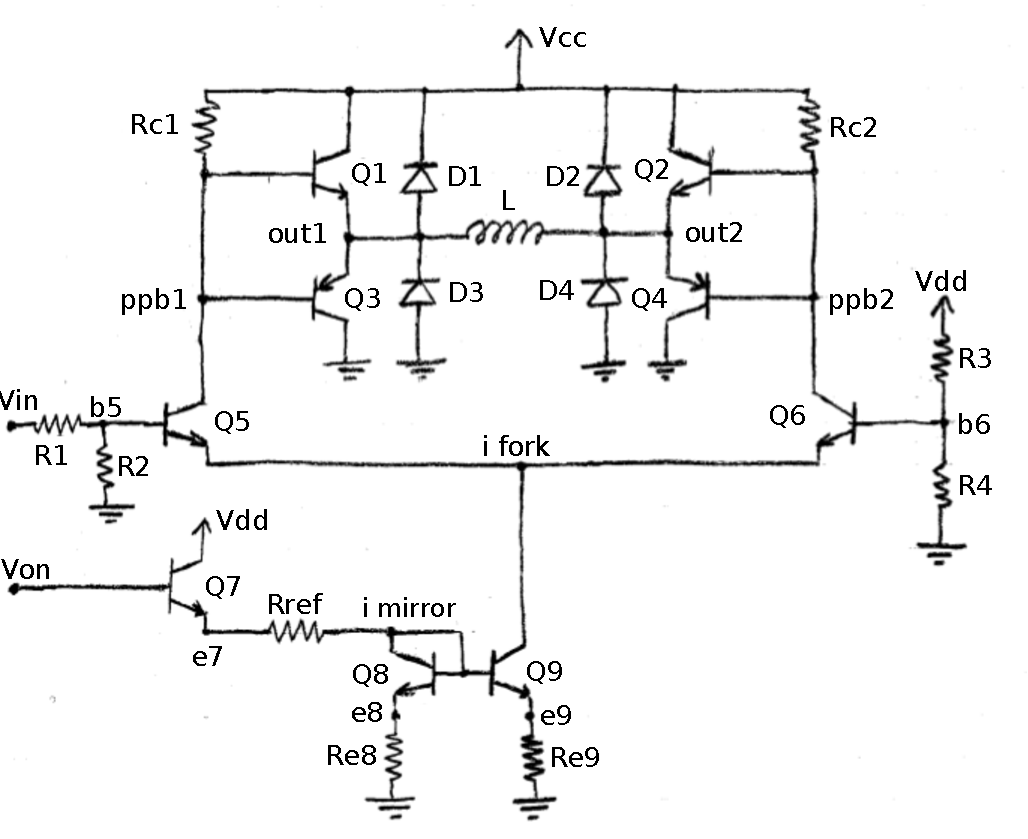
\includegraphics[width=.65\textwidth]{Figures/motor-driver-circuit.pdf}
	\caption{Push-Pull Driver Circuit for a Bipolar Motor}
	\label{motor-driver-circuit}
\end{figure*}

Only one of the power transistors ($Q_{1-4}$) on each vertical control line
will be on at any time, so the max base current for each vertical control line is
\begin{equation*}
I_{HB(max)}=\frac{I_{(sat)}}{h_{fe(min)}},
\end{equation*}
where $h_{fe(min)}$ for the MJE3x0 power transistors is 30 and $I_{(sat)}$ comes
is the motor's rated current.

If possible, based on the maximum power dissipation of the differential transistors
($Q_{5,6}$), the vertical control lines quiescent currents should be
\begin{equation}
\begin{array}{c}
I_{CQ}=10*I_{HB(max)},\quad\textrm{or}\\
I_{CQ}=\frac{P_{max(Q5,6)}}{V_{cc}-1.4\,V},
\end{array}
\label{vertical-control-line-quiescent-current}
\end{equation}
if $P_{max(Q5)}$ is the more limiting factor.

To set up the current mirror for the desired $I_{CQ}$ with $10\,\Omega$ emitter resistances,
the mirror ON voltages should be
\begin{equation}
V_{\textrm{imirror}}=10\Omega*I_{CQ}+0.7V,
\label{mirror-on-voltages}
\end{equation}
which is set by
\begin{equation*}
(V_{DD}-0.7V)-V_{\textrm{imirror}}=R_{ref}I_{CQ}
\end{equation*}
i.e.
\begin{equation}
R_{ref}=\frac{V_{DD}-1.4V}{I_{CQ}}-10
\label{Rref-eq}
\end{equation}

When the differential transistors ($Q_{5,6}$) are balanced,
they should both be biased fully on in saturation mode.
This is ensured with the approximate $V_{BE(on)}$ of 0.7 V and
a margin for error of 0.25 V.
\begin{equation*}
V_{B(\textrm{balanced})}=V_{\textrm{imirror}}+0.95\,V
\end{equation*}

The static bias network ($Q_{6}$) should be biased at the balance point
and the input bias network ($Q_{5}$) should swing above and below the
balance voltage with 0 and 5V inputs.
\begin{equation*}
V_{B(\textrm{balanced})}=\frac{R_{4}}{R_{3}+R_{4}}V_{DD}
\end{equation*}
\begin{equation*}
V_{B(\textrm{balanced})}+0.25\,V=\frac{R_{2}}{R_{1}+R_{2}}V_{DD}
\end{equation*}

For stiff bias, it is desirable that the total series resistance of
both bias networks is
\begin{equation*}
R_{\Sigma}\approx \frac{h_{fe(min)(Q5)}}{10}*\frac{V_{DD}}{I_{CQ}}
\end{equation*}

\begin{equation}
\begin{array}{r c l}
R_{1}	&=&	x\\
R_{2}	&=&	x\\
R_{3}	&=&	x\\
R_{4}	&=&	x\\
\end{array}
\label{Rbias12-eq}
\end{equation}

Two H--bridge networks are needed, but $R_{3}$ and $R_{4}$ do not
necessarily need to be repeated. If they are not, the $R_{\Sigma}$
for this network should be halved to support two base currents.

\begin{equation}
\begin{array}{r c l}
R_{3}	&=&	x\\
R_{4}	&=&	x\\
\end{array}
\label{Rbias34-eq}
\end{equation}

The collector resistors should be selected to allow maximum voltage
swing on the vertical control lines and be rated for the power
that may be dropped.
\begin{equation}
\begin{array}{c}
R_{Cx}=\frac{V_{CC}-V_{(\textrm{balanced})}}{I_{CQ}}	\\
P_{Rcx}\geq (V_{CC}-V_{(\textrm{balanced})})I_{CQ}
\end{array}
\label{Rcs-eq}
\end{equation}


\subsection{Driver SPICE Simulation}

The circuit in
\hyperref[motor-driver-circuit]{figure \ref{motor-driver-circuit}}
was simulated in SPICE with the net listed in
\hyperref[motor-driver-listing]{section \ref{motor-driver-listing}}.
Five volt step functions were applied to both $V_{on}$ and $V_{in}$ to simulate the microcontroller.
The results in 
\hyperref[motor-driver-voltage-simulation]{figure \ref{motor-driver-voltage-simulation}}
and
\hyperref[motor-driver-current-simulation]{figure \ref{motor-driver-current-simulation}}
show how motor loads the power supply.

\begin{figure}
	\centering
	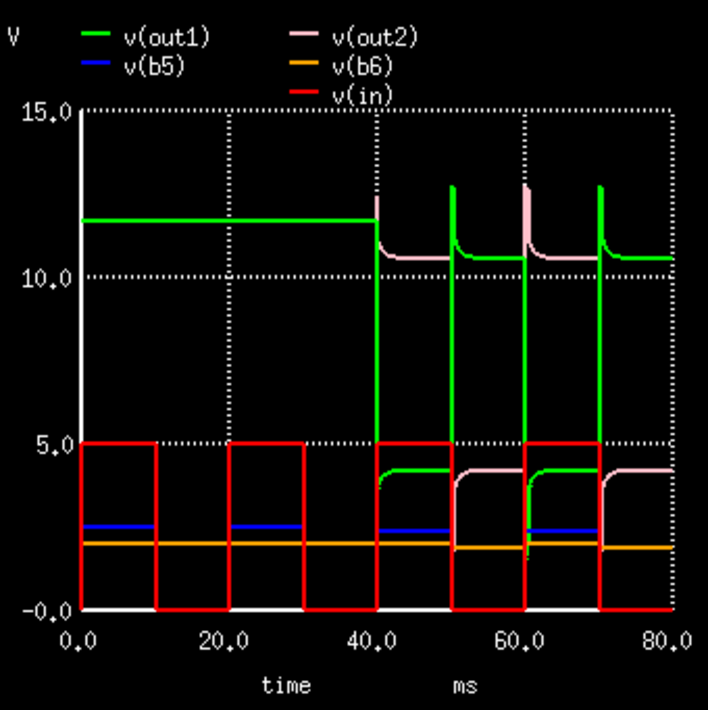
\includegraphics[width=0.75\columnwidth]{Figures/motor-driver-voltage-simulation.pdf}
	\caption{Simulated Voltages across One Driver}
	\label{motor-driver-voltage-simulation}
\end{figure}

\begin{figure}
	\centering
	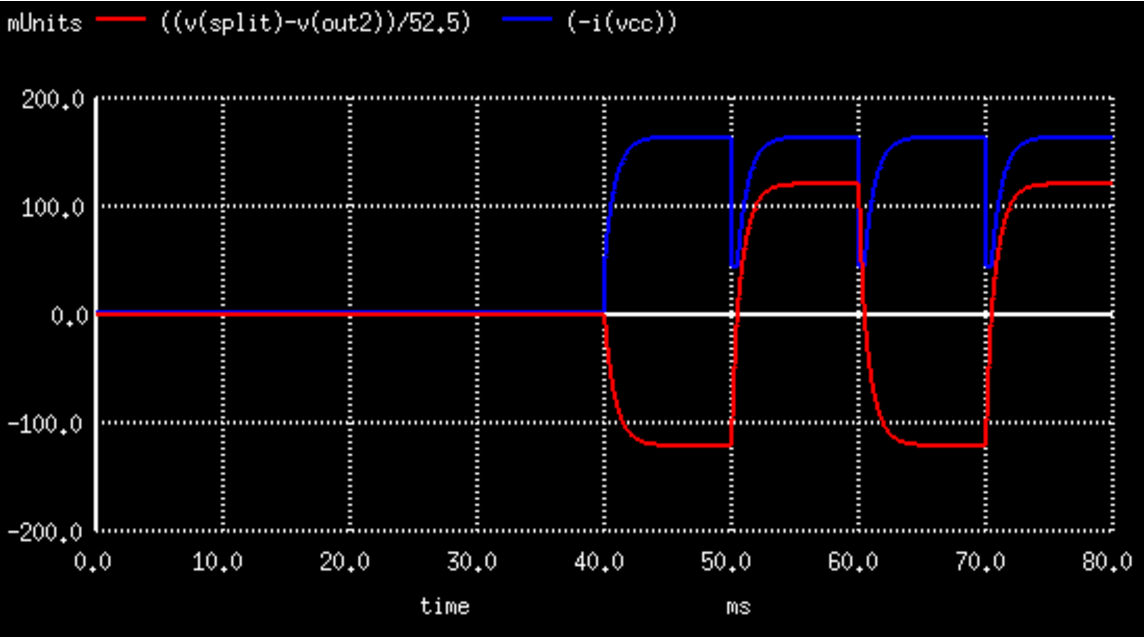
\includegraphics[width=0.9\columnwidth]{Figures/motor-driver-current-simulation.pdf}
	\caption{Simulated Current through One Driver}
	\label{motor-driver-current-simulation}
\end{figure}

\section{Heat Relay Design}

\begin{figure}
	\centering
	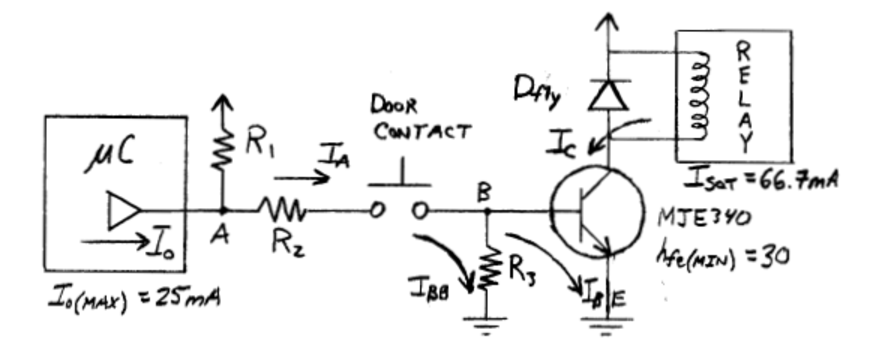
\includegraphics[width=\columnwidth]{Figures/relay-drive-circuit.pdf}
	\caption{Heat Relay Drive Cicuit and Door Safety Switch}
	\label{relay-drive-circuit}
\end{figure}

\subsection{Door Contact Safety Switch}

The drive circuit for operating the heat relay is shown in
\hyperref[relay-drive-circuit]{figure \ref{relay-drive-circuit}}.
The switch shown in a form A contact block that is mounted on the front--facing PCB
and closes when the oven door closes. With this safety switch,
the microcontroller cannot turn the heating element on when the door is open.

To allow the $\mu$Controller to sense the switch's state, a pullup resistor is added.
In order to ignore the pullup resistor when designing the transistor bias network,
the pullup should be an order of magnitude greater than the BJT base bias network.
\begin{equation}
R_{1}\approx 10*R_{2}
\label{heat-relay-pullup-eq}
\end{equation}

\subsection{Relay \& Components Selection}

The Omron G5LE--1A--E relay is rated for switching voltages up to 250 VAC
with a contact rating of 16 A. 

For the driver circuit in
\hyperref[relay-drive-circuit]{figure \ref{relay-drive-circuit}},
the amplifier BJT and flyback diode should be rated for currents
greater than the saturation current of the relay coil,
which is $33.3\,mA$ at $12\,V$ for the G5LE--1A--E.

The flyback diode should be rated for power dissipation greater than
\begin{equation*}
P_{\textrm{diode}}>33.3\,mA*12\,V=400\,mW.
\end{equation*}

The BJT should be sized for continuous collector saturation current greater than
\begin{equation}
I_{c(sat)}>I_{\textrm{relay}(sat)}=33.3\,mA
\end{equation}

\subsection{Relay Driver Design}

When the relay is on, the maximum possible current drawn through the
base depends upon the maximum possible coil saturation current of the relay
and the minimum possible base--collector current gain of the BJT.
For the MJE340 NPN BJT,
\begin{equation*}
I_{B(max)}=\frac{I_{C(sat)}}{h_{fe(min)}}=\frac{33.3\,mA}{30}=1.11\,mA
\end{equation*}

The total current from the microcontroller when the heater is on should
be be somewhat greater than 1.11 mA to reduce the impact of variation in
transistor $h_{fe}$, but less than the 25 mA limit of the $\mu$Controller.
If we choose $4\,mA$, then
\begin{equation}
\left\{\begin{array}{c c c}
V_{A(on)}	&=&	I_{0(on)}R_{2}+V_{B(on)}	\\
V_{B(on)}	&=&	(I_{0(on)}-I_{B(max)})R_{3}	\\
\end{array}\right.
\label{heat-relay-bias-network-eq}
\end{equation}

\begin{equation*}
\left\{\begin{array}{c c c}
V_{A(on)}	&=&	(4\,mA)R_{2}+V_{B(on)}	\\
V_{B(on)}	&=&	(4-1.11\,mA)R_{3}	\\
\end{array}\right.
\end{equation*}

Choosing 1 V for $V_{B(on)}$ provides some margin for error compared to $V_{BE(on)}\approx 0.7\,V$.
Using this with equations
\ref{heat-relay-pullup-eq} and \ref{heat-relay-bias-network-eq}
defines the resistor values for relay driver network.

\begin{equation}
\begin{array}{c c c}
R_{1}	&=&	10\,k\Omega	\\
R_{2}	&=&	1\,k\Omega	\\
R_{3}	&=&	333\,\Omega	\\
\end{array}
\end{equation}

\section{Power Circuit Design}

\subsection{Safety \& Supply Requirements}

The power circuit is responsible for switching on and off 120 VAC power
to the nichrome heating element; for converting 120 VAC to 12 and 5 volt
supplies; and for protecting against faults and surges for safety.
Current requirements for the most power hungry components are summarized in
\hyperref[current-requirements-table]{table \ref{current-requirements-table}}.

\begin{table}
	\centering
	\small
	\caption{Current Requirements}
	\begin{tabular}{c c c}
		\hline\hline
		Component					&Voltage	&Current	\\
		\hline
		135 ft, 0.051" $\emptyset$ nichrome wire	&120 VAC	&3.43 A	\\
		bipolar motor driver		&12 VDC		&400 mA	\\
		SPST form A Relay				&12 VDC		&67 mA	\\
		LED display driver				&5 VDC		&200 mA	\\
		Op Amp quiescent current			&5 VDC		&25 $\mu$A	\\
		PIC16F833 supply current			&5 VDC		&1 mA	\\
		\hline\hline
	\end{tabular}
	\label{current-requirements-table}
\end{table}

\subsection{Power Circuit Topology}

\begin{figure*}
	\centering
	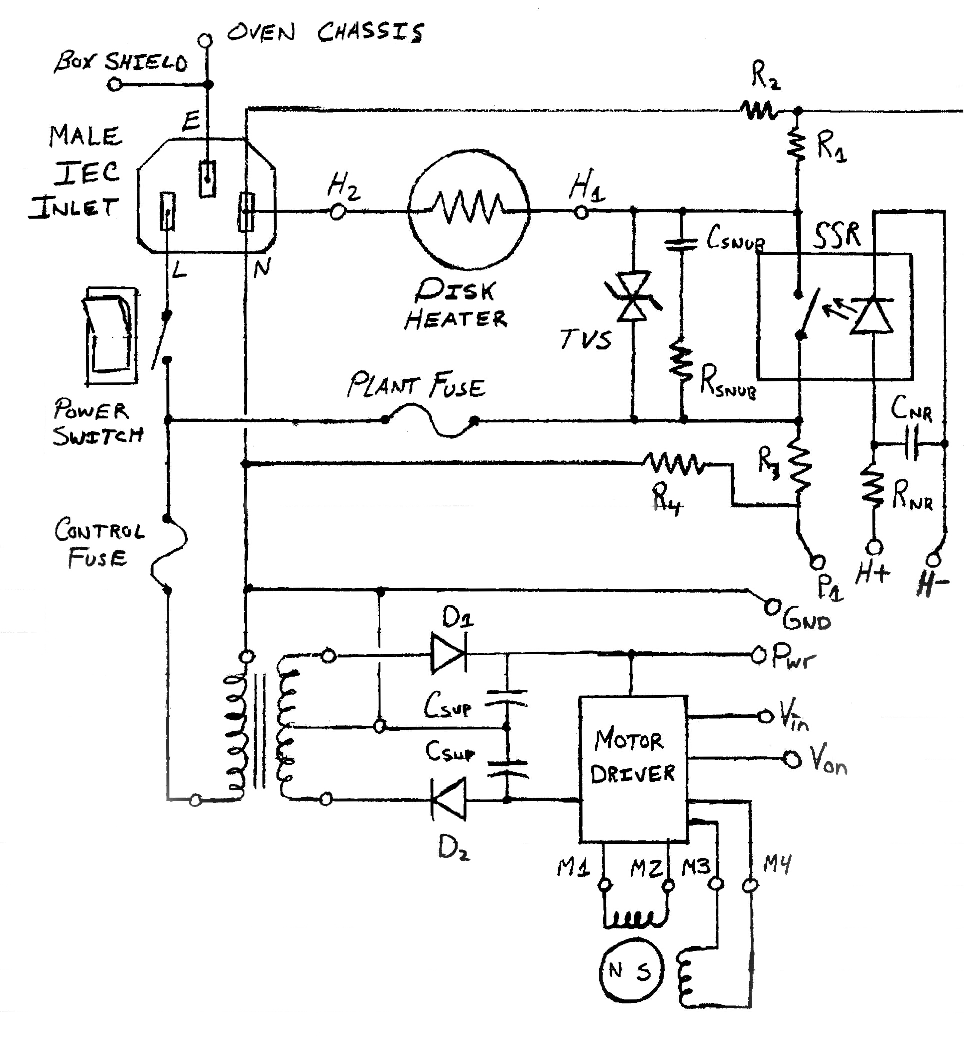
\includegraphics[width=0.75\textwidth]{Figures/power-circuit.pdf}
	\caption{Power Circuit Design}
	\label{power-circuit}
\end{figure*}

The nichrome wire is exposed to improve thermal conductivity with the air.
Unfortunately it is also exposed electrically, with 120 VAC coursing through
it when on. If a fault occured at the half way point, as much as 7 Amps could
pass through the metal or human that touched the wire.

To protect against electric faults, the power circuit will include fuses
on both live and neutral power lines and a ground fault circuit interuptor
wall adapter must be used. The power circuit will include a power
switch close to the inlet and the relay actuating the nichrome wire will
be form A so that by default it is open.

A center tapped transformer will be used to produce the 12 V and 5 V supplies.
The transformer and the form A relay with resistive load are
inherently strong against electric surges.

Downline of the transformer are two bridge rectifiers, two ripple capacitors,
and for the 5 V supply a voltage regulator.

The power circuit with all these features is shown in
\hyperref[power-circuit]{figure \ref{power-circuit}}.

\subsection{Power Circuit Design}

\subsection{PCB Trace Width}

To reduce the chances of faults due to wiring/assembly, most of the power
circuit will be mounted on a PCB with an IEC inlet port and screw terminal
blocks for wires that must head into the oven frame.

For the PCB, the minimum width and clearance for high current,
high voltage traces can be calculated using
\begin{equation}
I=0.048[A]*\left(\frac{\Delta T}{[^{o}C]}\right)^{0.44}*\left(\frac{A}{[mil^{2}]}\right)^{0.725}
\label{trace-width-eq}
\end{equation}
and
\begin{equation}
\textrm{Clearance}=0.023[in]+\frac{0.0002[in]}{[V]}*V_{\textrm{peak}}
\end{equation}
from the design standard for PCB trace width ANSI/IPC--2221. Note that
equation \ref{trace-width-eq} is only for exterior traces.

For $10\,A$, $120\,VAC$ power with a maximum temperature rise of $10^{o}C$
and standard copper thickless $1\,oz=1.4\,mil$, the minimum trace width
is $0.278\,in$ and minimum clearance is $0.057\,in$.

\section{Controller Design}
\label{controller-section}

\subsection{PIC Requirements \& Circuit}

\begin{figure}
	\centering
	\includegraphics[width=\columnwidth]{Figures/controller-pcb.pdf}
	\caption{Oven Controller Board}
	\label{controller-pcb}
\end{figure}

The controller PCB is shown in
\hyperref[controller-pcb]{figure \ref{controller-pcb}}.
At its heart is a 28--pin, DIP, 5V, \textrm{PIC16F883} $\mu$Controller.
It has all of the requirements for  \textrm{Easy--PCB}:
3+ channels of ADC, two PWM modules, SPI, USART, and 10+
digital I/O with at least one external interupt.
The mapping of the pins on the \textrm{PIC16F883} is shown in
\hyperref[pic16f883-circuit]{figure \ref{pic16f883-circuit}}.

\begin{center}
	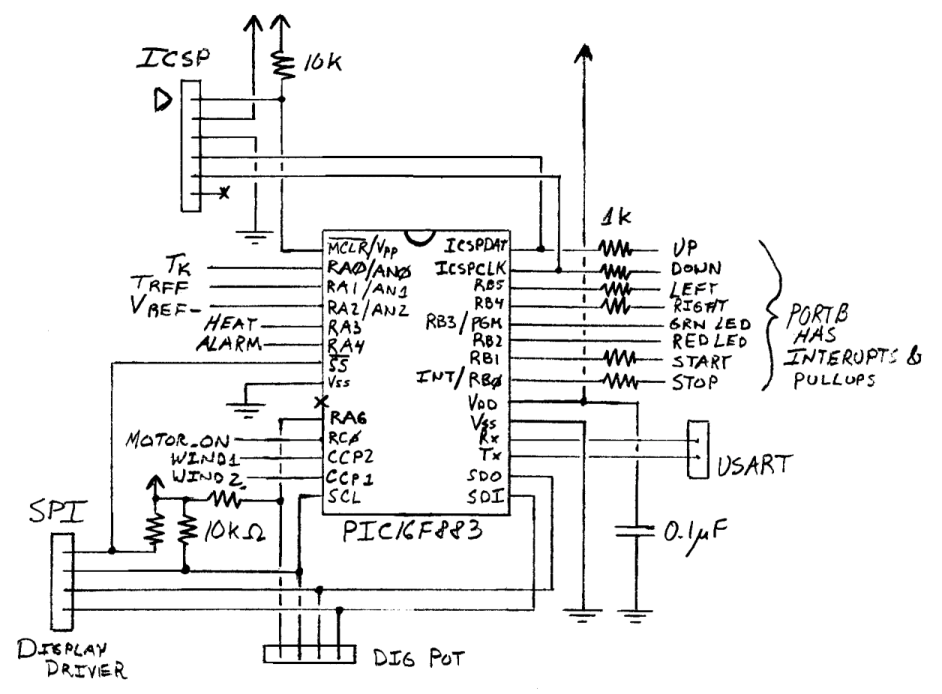
\includegraphics[width=\columnwidth]{Figures/pic16f883-circuit.pdf}
	\captionof{figure}{\textrm{PIC16F883} Pinout Diagram}
	\label{pic16f883-circuit}
\end{center}

\subsection{Interupts and Safety}

\subsection{Memory Organization}

\subsection{Timing Design}

\subsection{Program Flowcharts}

An overall flowchart is shown in figure
\ref{high-level-program-flowchart}.

\begin{figure*}
	\centering
	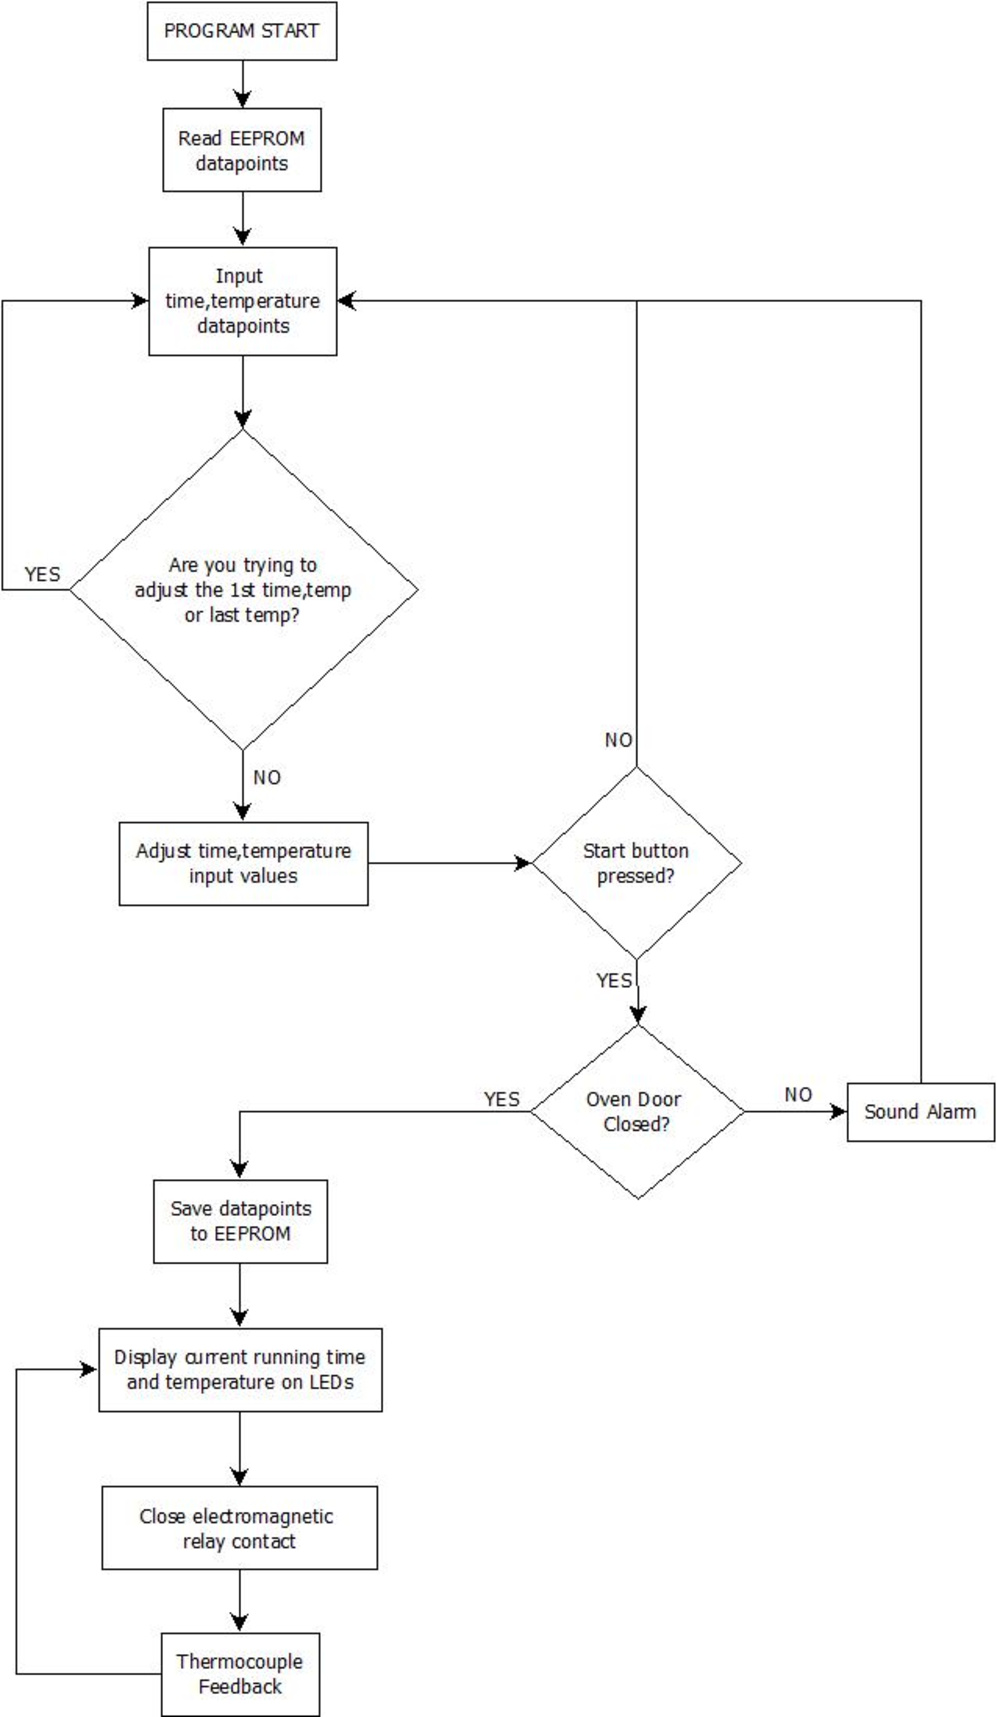
\includegraphics[width=0.75\textwidth]{high-level-program-flowchart.pdf}
	\caption{High Level Program Flowchart}
	\label{high-level-program-flowchart}
\end{figure*}

The program is separated into two logical halves:
the user interface loop and the control loop.
Pressing start from the user interface loop causes the
program to enter the control loop.
Pressing stop at any time triggers an interupt which
restarts the user interface loop.

The user interface loop is shown in
\hyperref[user-interface-flowchart]{figure \ref{user-interface-flowchart}}
and the control loop is shown in
\hyperref[control-flowchart]{figure \ref{control-flowchart}}.

Initialization and several subfunctions are depicted in figures
\ref{user-interface-flowchart-1},
\ref{user-interface-flowchart-2},
\ref{user-interface-flowchart-3}, and
\ref{user-interface-flowchart-4}.

\begin{figure*}
	\centering
	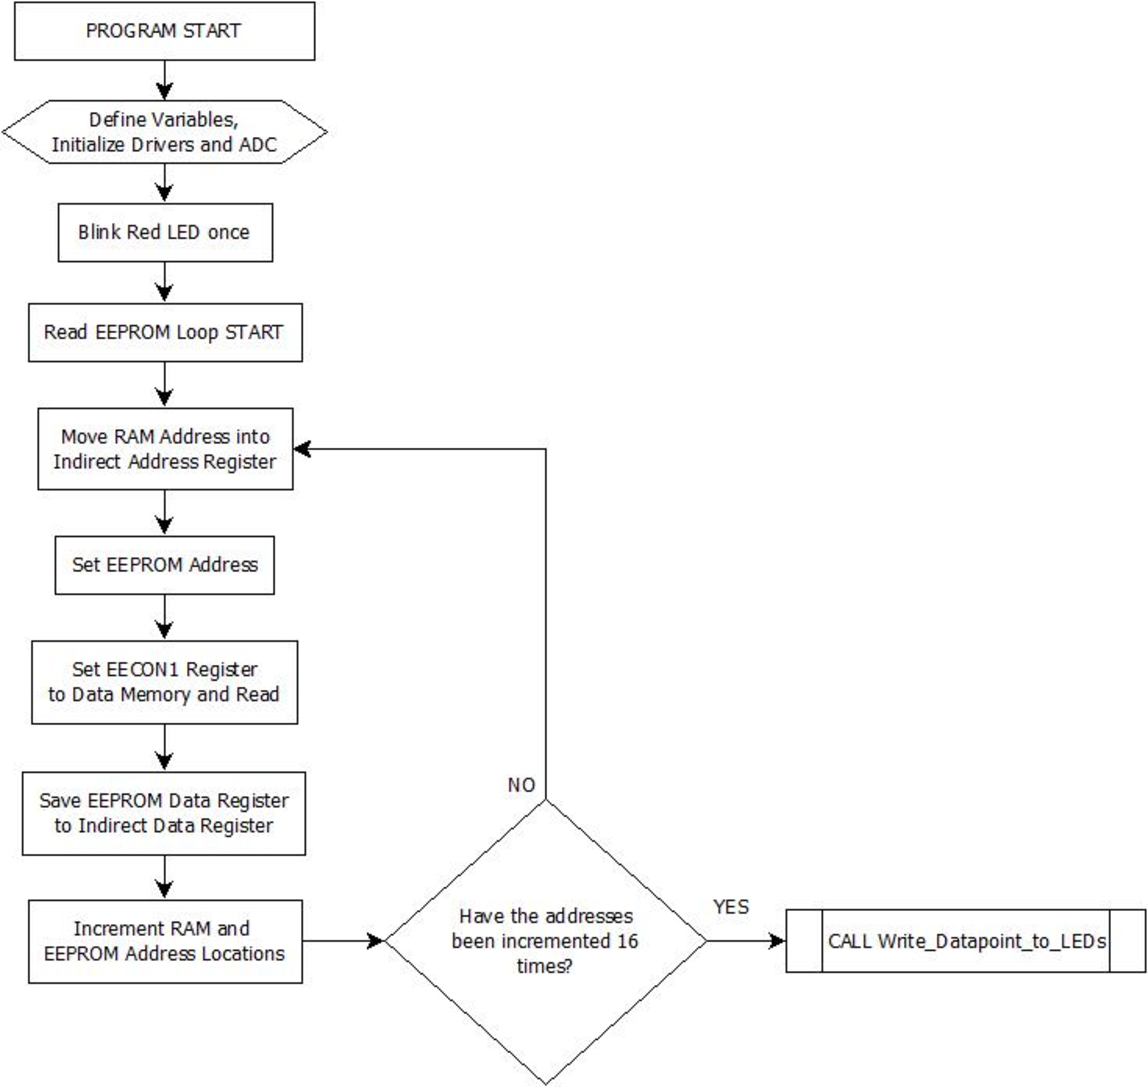
\includegraphics[width=1\textwidth]{Figures/user-interface-flowchart.pdf}
	\caption{User Interface Program Flowchart}
	\label{user-interface-flowchart}
\end{figure*}

\begin{figure*}
	\centering
	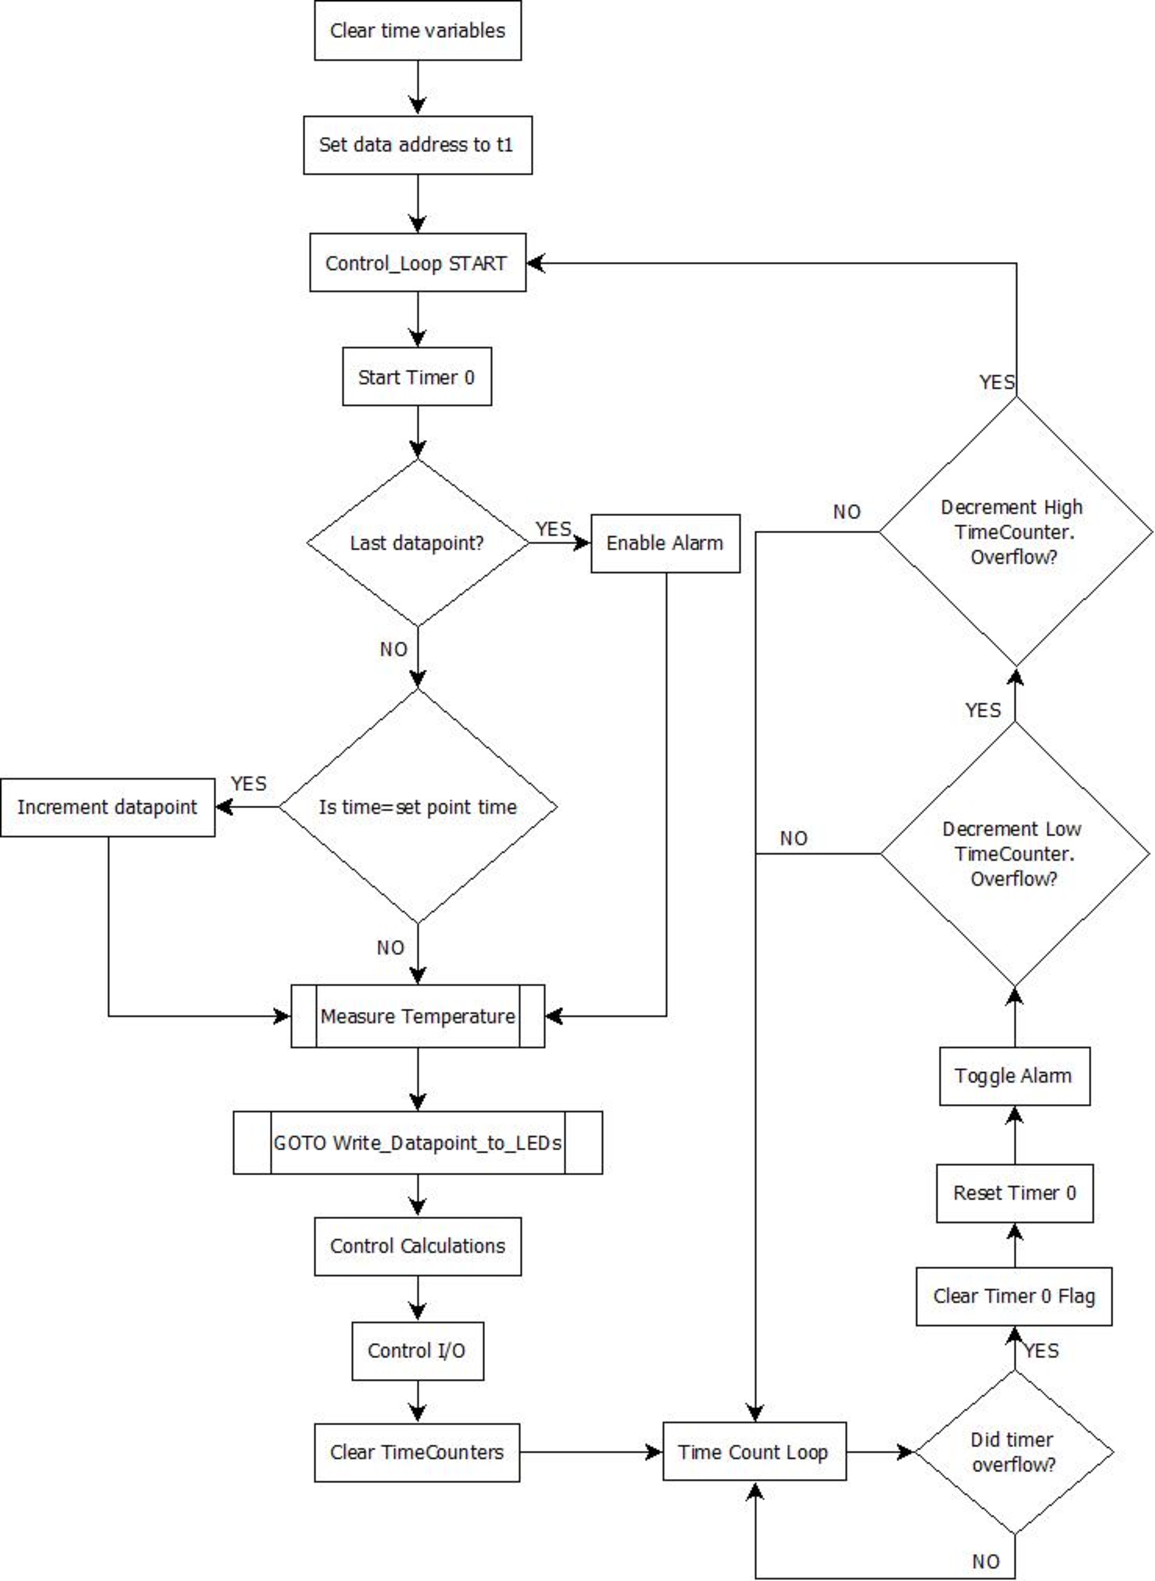
\includegraphics[width=\textwidth]{Figures/control-flowchart.pdf}
	\caption{Runtime Control Program Flowchart}
	\label{control-flowchart}
\end{figure*}

\begin{figure}
	\centering
	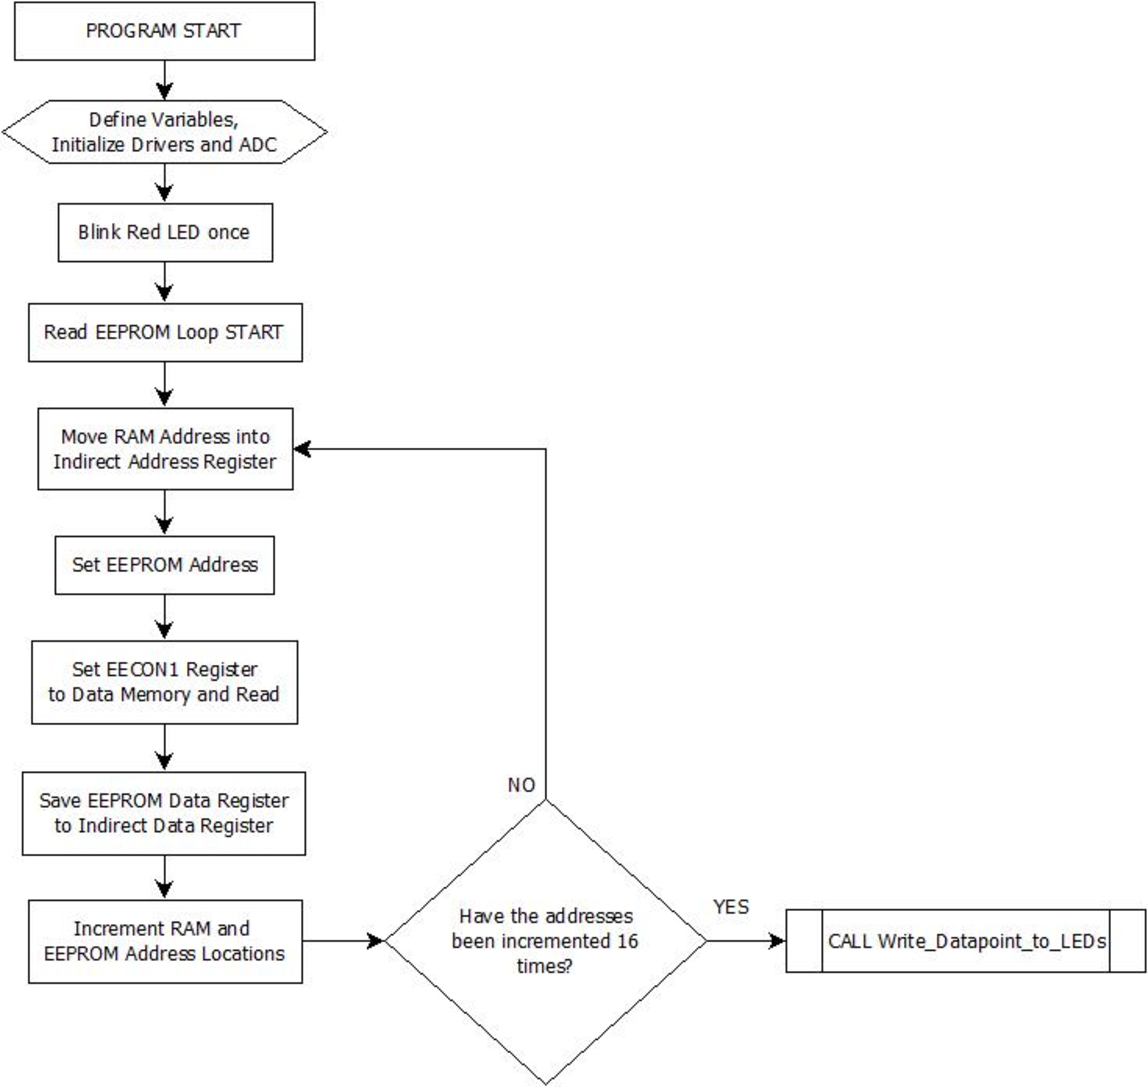
\includegraphics[width=\columnwidth]{user-interface-flowchart-1.pdf}
	\caption{Program Initialization Flowchart}
	\label{user-interface-flowchart-1}
\end{figure}

\begin{figure*}
	\centering
	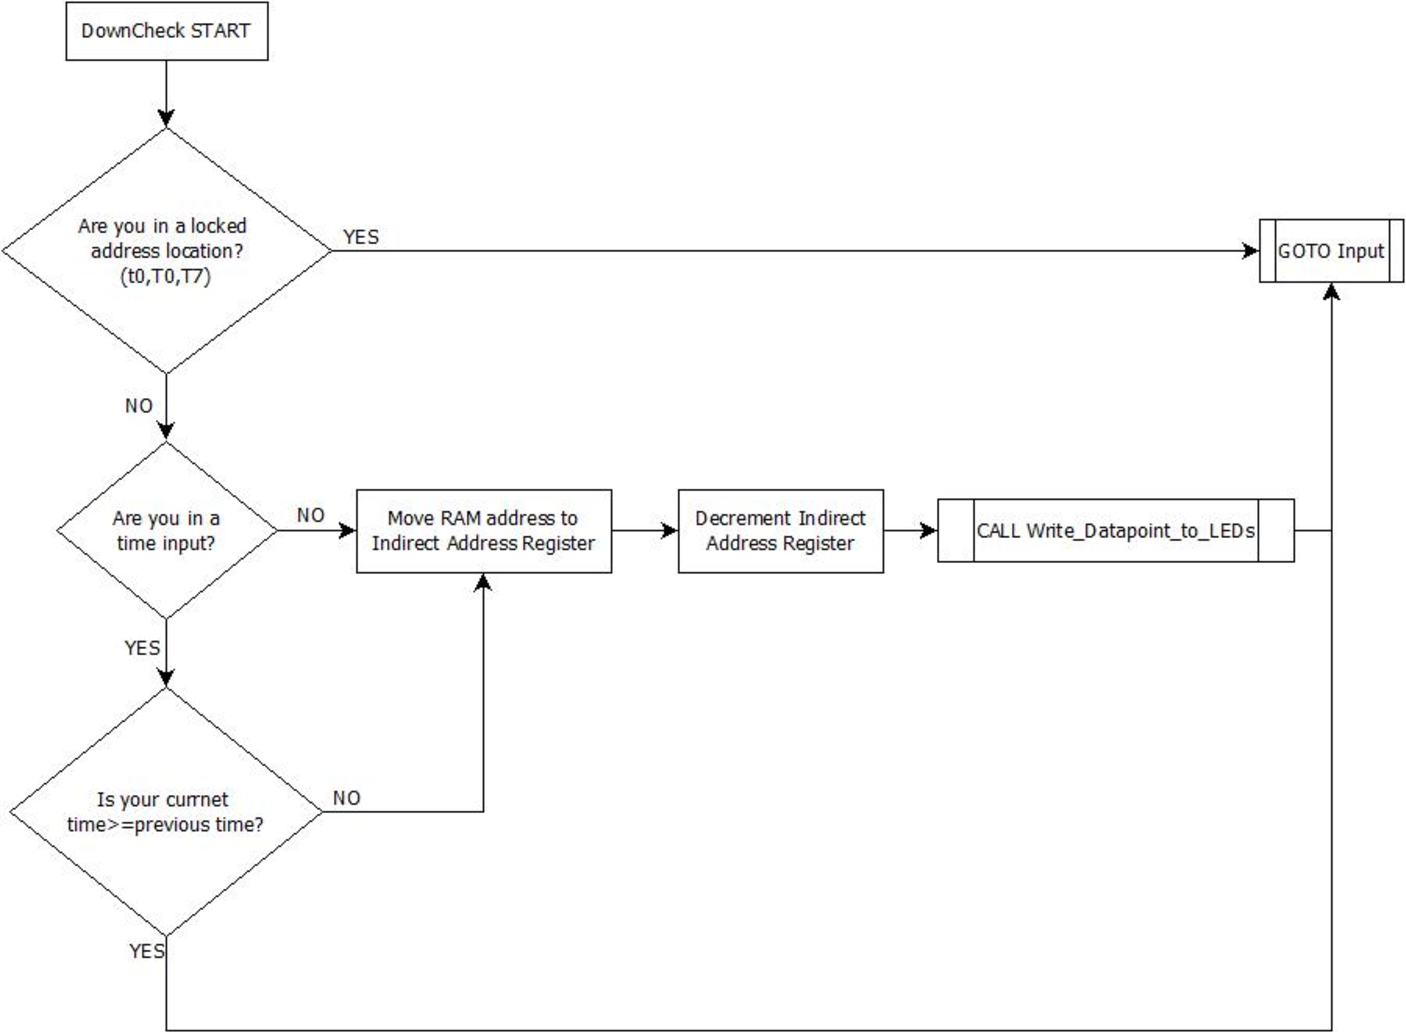
\includegraphics[width=0.75\textwidth]{user-interface-flowchart-2.pdf}
	\caption{Down Button Subroutine}
	\label{user-interface-flowchart-2}
\end{figure*}

\begin{figure*}
	\centering
	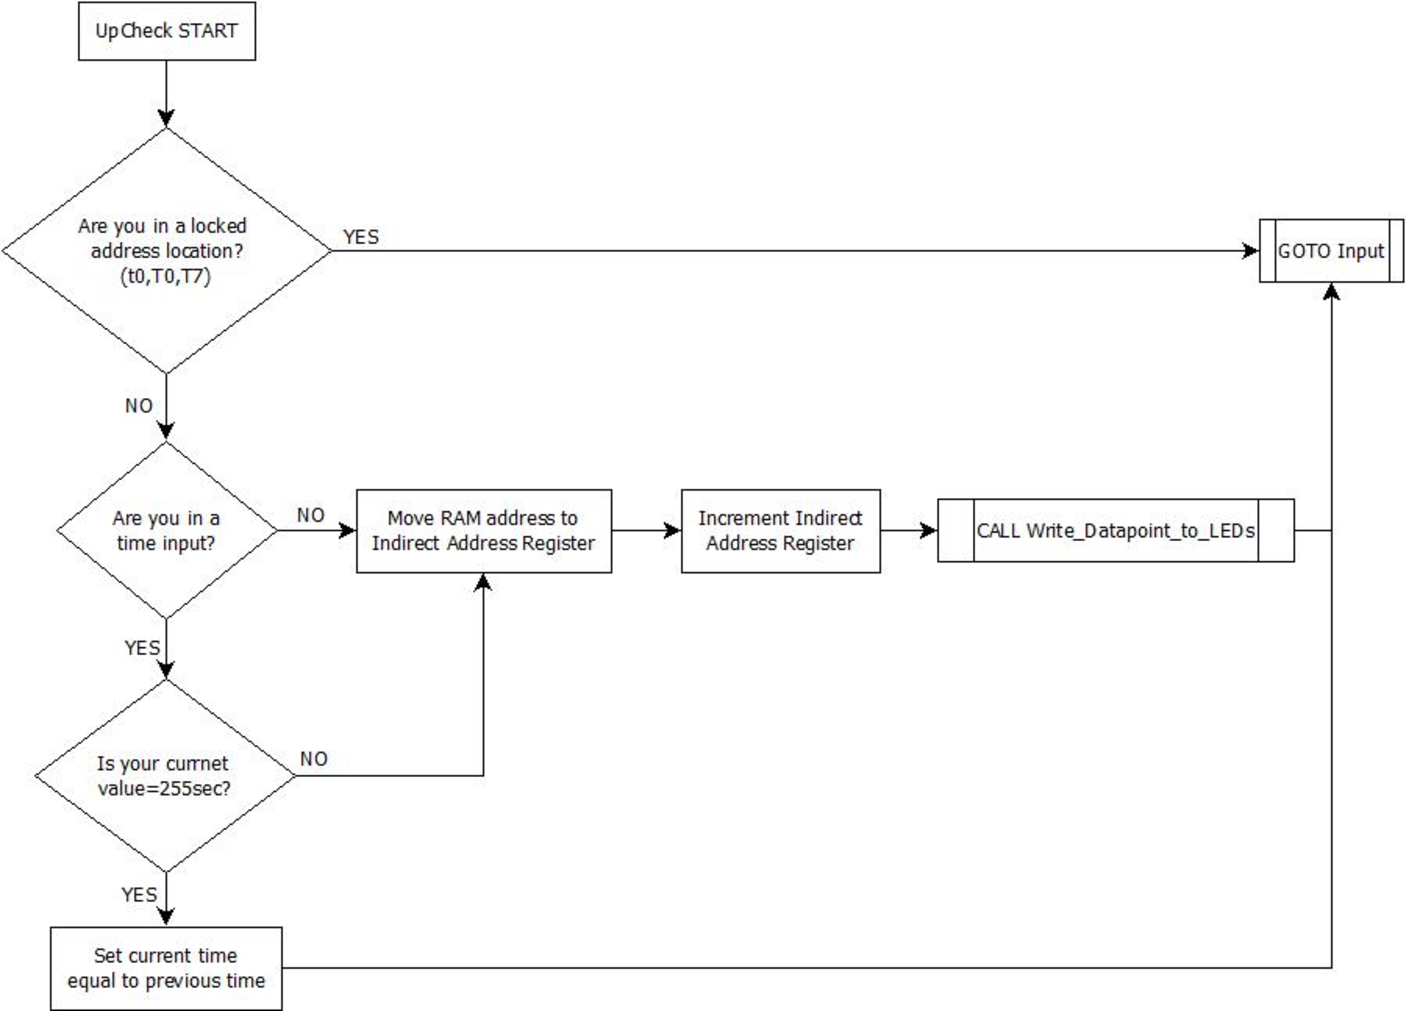
\includegraphics[width=0.75\textwidth]{user-interface-flowchart-3.pdf}
	\caption{Up Button Subroutine}
	\label{user-interface-flowchart-3}
\end{figure*}

\begin{figure}
	\centering
	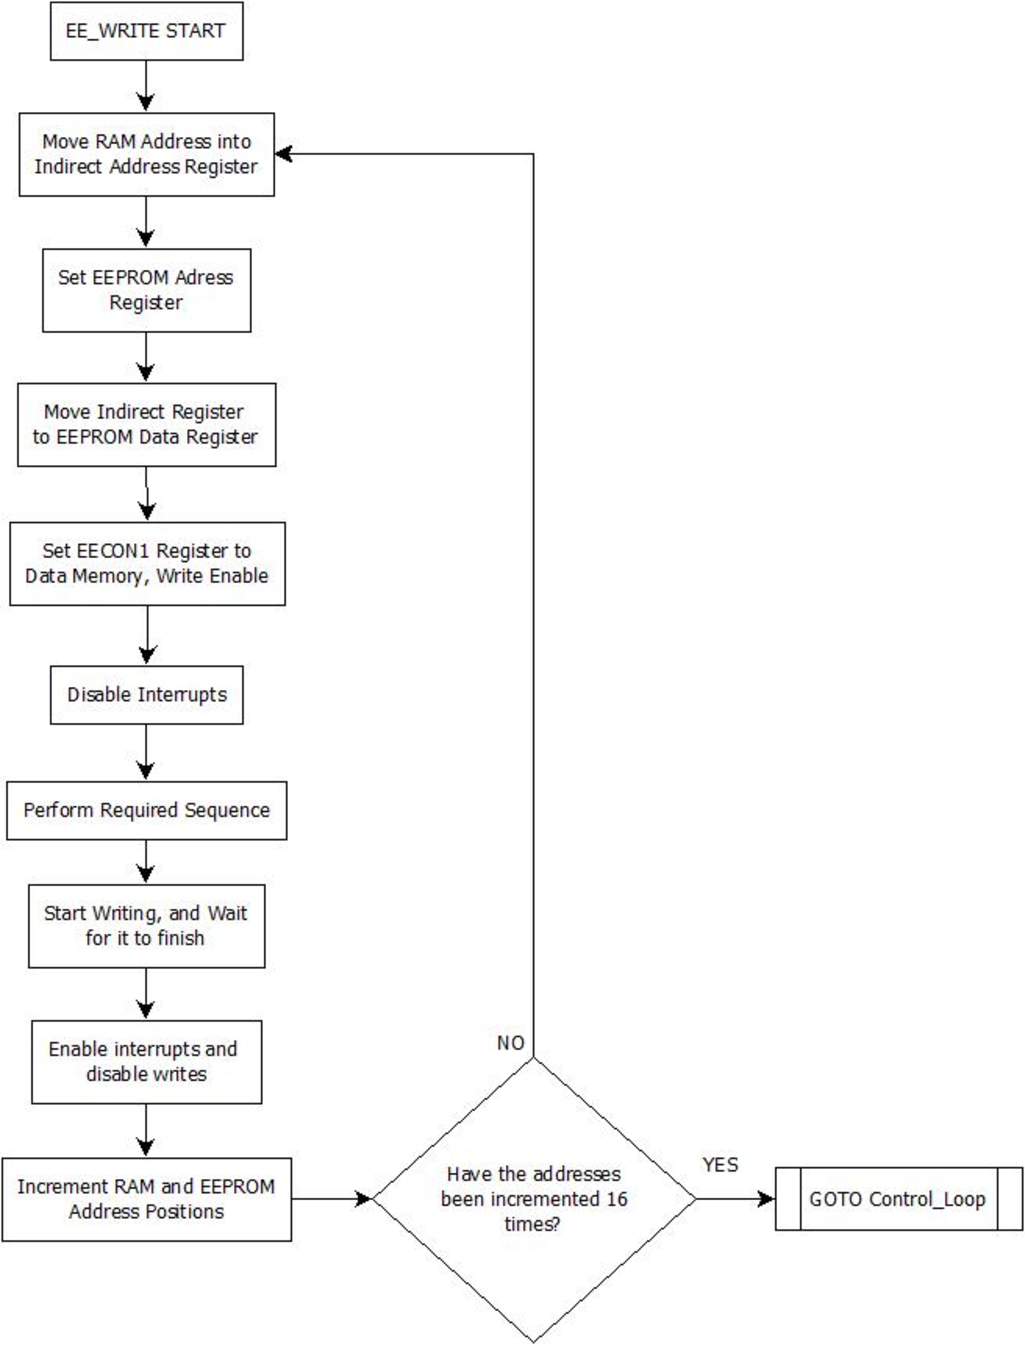
\includegraphics[width=\columnwidth]{user-interface-flowchart-4.pdf}
	\caption{EEPROM Write Subroutine}
	\label{user-interface-flowchart-4}
\end{figure}

The program itself is listed in
\hyperref[easy-pcb-listing]{appendix \ref{easy-pcb-listing}}.

\subsection{Control System Design}

\section{Additional Items for the Final Report}

\subsection{System in Action}

The following features are implemented on
our demo breadboard:
\begin{enumerate}
\item LED display
\item User interface with set point programming of up to 8 points
\item Safety interupt with stop button
\item EEPROM reading and writing
\item Timer 0 and the beginning of the control loop
\item Piezo Alarm (without masking yet)
\item Thermocouple amplifier circuit
\item Heat relay circuit is tested but not a part of the program yet
\end{enumerate}

Photos of the system in action are shown in figures
\ref{controller-pcb} and \ref{front-facing-pcb}. The two
circuits shown are connected by a 1ft ribbon cable.
We were able to implement all of the parts of the black box diagram
(figure \ref{detailed-system-diagram}) that were driven by 5 Volts
and also the relay which was driven by 12 V.

Left unfinished were the motor driver, the power circuit, and the
actual control algorithm.

\subsection{Final Test Plan}

We were able to test the temperature feedback monitoring by using
the thermocouple in the kitchen oven. The results of this test are
shown in figure \ref{temperature-control-results}.

Once I construct the oven in the machine shop next week,
I will be able to begin testing of the power circuis and see if the heat 
transfer design model is correct.

Once I have some real temperature and heating data, I will develop a control
algorithm that is probably a PI or PID controller.

\subsection{Bugs Discovered}

Over the course of building our device, we encountered four issues.
Three of these issues were related to the programming, while the last was hardware.

The first programming bug involved the pushbutton I/O pins.
The pins are analog or digital, but the default is analog.
To remedy this, we needed to set the pins for digital inputs in order for the pushbuttons to register with the microcontroller.

The next programming bug caused a reset every time anything other than zero
was going to be displayed on the LEDs.
The error was occurring in the LED lookup table due to invalid values being
used to call selections from the lookup table.
This error bug was corrected by revising the Update LED Display routine to output valid values to the lookup table.

The last programming bug was an error adjusting the frequency for the alarm.
The alarm goes off when timer0 overflows, however the frequency is adjusted
in a different bank than timer0. The solution was to select the correct bank for frequency adjustment.

The only hardware issue we encountered was in the op-amp circuit for the thermocouple.
We set the op-amp up in an inverting configuration but we didn’t have a negative voltage source.
The remedy was to make the op-amp non-inverting and use a negative reference voltage on the
opamp and the PIC.

\onecolumn
\appendix

\section{SPICE Netlists}

\subsection{Thermodynamic Model}
\label{heat-model-listing}
\lstinputlisting[basicstyle=\small]{NGSPICE/Thermo/heat-model.cir}

\subsection{Bipolar Motor Driver}
\label{motor-driver-listing}
\lstinputlisting[basicstyle=\small]{NGSPICE/Motor-Driver/motor-driver.cir}

\pagebreak
\section{PIC Assembly Listings}

\subsection{easy--pcb.asm}
\label{easy-pcb-listing}
\lstinputlisting[basicstyle=\small]{PIC-Program/easy-pcb.asm}

\pagebreak
\section{Bill of Materials}

\begin{center}
\captionof{table}{Digi--Key Bill of Materials}
\begin{adjustbox}{max width=\textwidth}
\begin{tabular}{c c c c c c c c c c}
\hline\hline
Item	&Qty	&Labels	&Description		&Electrical Specs		&Mechanical Specs
	&Manufacturer		&Part Number		&Unit Cost	&Total Cost	\\
\hline

	&1	&RP1	&8 resistor array	&8 x $320\,\Omega$		&DIP
	&Bourns Inc.		&4116R-1-331LF		&0.76		&0.76		\\

	&1	&R24	&Relay voltage drop	&$330\,\Omega$, $\geq 0.5\,W$	&
	&Yageo			&FMP100JR-52-330R	&0.15		&0.15		\\

	&1	&R25	&$V_{DD}$ supply LP filter	&$10\,\Omega$, $\geq 2\,W$	&
	&TE Connectivity	&1625890-6		&0.20		&0.20		\\
	
	&2	&R26,28	&Motor Driver	&$140\Omega$, see eq. \ref{Rbias12-eq}	&
	&			&			&		&		\\

	&2	&R27,29	&Motor Driver	&$115\Omega$, see eq. \ref{Rbias12-eq}	&
	&			&			&		&		\\

	&2	&R30,31	&Motor Driver	&$64\Omega$, see eq. \ref{Rbias34-eq}	&
	&			&			&		&		\\

	&4	&R32--35	&Motor Driver	&$165\Omega$, $P\geq 0.6W$, see eq. \ref{Rcs-eq}	&
	&Yageo			&RSF100JB-73-160R	&0.25		&1.00		\\

	&1	&R36	&Motor Driver		&$51\Omega$, see eq. \ref{Rref-eq}
	&			&			&		&		\\

	&3	&R37--39	&Motor Driver	&$10\Omega$		&
	&			&			&		&		\\


1	&4	&	&navigation pushbuttons	&SPST				&17.3 dist. PCB to enclosure
	&E-Switch		&RP3502BBLK		&2.04		&8.16	\\

2	&1	&	&green “start” button	&SPST switch/1.8V, 20mA LED	&18 mm dist. PCB to enclosure
	&E-Switch		&RP3508BBLKGRNGRNNS	&5.43		&5.43	\\

3	&1	&	&red “stop” button	&SPST switch/1.8V, 20mA LED	&18 mm dist. PCB to enclosure
	&E-Switch		&RP3508BBLKREDREDNS	&5.43		&5.43	\\

4	&1	&	&door contact block	&SPDT, momentary		&
	&Apem Inc.		&A0151B			&6.76		&6.76	\\

5	&6	&	&pushbutton I limiters	&1kOhm				&
	&		&			&		&	\\

6	&1	&	&Rset for LED display driver	&10 kOhms, 5\% tolerance	&
	&		&			&		&	\\

7	&2	&	&SW5,6 LED I limiters	&500 Ohms			&
	&		&			&		&	\\

8	&2	&	&SPI pull ups		&50 kOhms			&
	&		&			&		&	\\

9	&1	&	&7--seg, 8--dig disp. driver	&com.--cathode, SPI, 5V, 333 mA	&"0.1” pitch, DIP
	&Maxim Integrated	&MAX7219CNG		&9.13		&9.13	\\

10	&1	&	&24--pin, DIP Socket	&				&.1” pitch, 0.3” row spacing
	&3M		&4824-3000-CP			&0.74		&0.74	\\

11	&1	&	&7-seg, LED clock display	&com.-cathode	&0.1” pitch, DIP"
	&Lite--On Inc.		&LTC-4727JR		&3.56		&3.56	\\

12	&1	&	&decoupling capacitor	&0.1uF				&
	&		&				&		&	\\

13	&2	&J3,	&front PCB to controller PCB	&20 pos			&1mm pitch, 1 row flat flex
	&FCI			&HLW20R-2C7LF		&0.21		&0.42	\\

14	&1	&	&12” flat flex ribbon		&20 pos		&1mm pitch, 1 row
	&Parlex USA LLC		&100R20-305B		&6.08		&6.08	\\

15	&1	&SP1	&2 kHz piezo buzzer	&5V(0-peak)			&
	&TDK Corporation	&PS1420P02CT		&0.85		&0.85	\\

16	&2	&R14,15	&piezo resistors	&1kOhm				&
	&			&			&		&	\\

17	&1	&Q1	&piezo drive BJT		&NPN				&
	&Fairchild Semiconductor	&2N3904BU	&0.18		&0.18	\\

18	&1	&	&type--K thermocouple	&				&
	&			&			&		&	\\

19	&1	&U4	&thermocouple Op Amp	&$V_{out}=\pm 20\,mV$ of supply	&8--pin, 0.1” DIP
	&Microchip Technology	&MCP617--I/P		&1.02		&1.02	\\

20	&1	&U3	&cold jnct temp. sensor	&Vout=500mV + 10mV/degC 	&-40 to 125$^{o}C$
	&Microchip Technology	&MCP9700--E/TO		&0.31		&0.31	\\

21	&1	&	&Bipolar Stepper Motor	&12 V, 350 mA		&5 mm $\emptyset$ Shaft, $42x42\,mm^{2}$ body, M3 mounts
	&Adafruit		&324			&14.00		&14.00	\\

22	&4	&	&crimp socket connectors	&			&for 24--30 AWG
	&Molex, LLC		&0016020069		&0.12		&0.48	\\

23	&1	&	&4--pos. connector housing	&			&0.1'' pitch
	&Molex, LLC		&0050579004		&0.46		&0.46	\\

24	&1	&	&4--pos. male header	&				&0.1'' pitch, tin
	&Molex, LLC		&0022032041		&0.32		&0.32	\\

22	&4	&Q1,2,11,12	&NPN BJTs for H--bridge	&$I_{c(max)}>171\,mA$, $P_{max}>2\,W$	&
	&Fairchild Semiconductor	&MJE340STU	&0.50		&2.00	\\

23	&4	&Q3,4,13,14	&PNP BJTs for H-bridge	&$I_{c(max)}>171\,mA$, $P_{max}>2W$	&
	&Fairchild Semiconductor	&MJE350STU	&0.42		&1.68	\\

24	&8	&D1--8	&H--bridge flybacks	&$V_{R}\geq1\,kV$, $I_{0}\geq 1\,A$	&
	&Diodes Incorporated	&1N4007--T		&0.13		&1.04	\\

25	&8	&	&H--bridge control	&NPN, 2N3904			&
	&Fairchild Semiconductor	&2N3904BU	&0.18		&1.44	\\

26	&4	&	&H--bridge Rcs			&					&
	&			&			&		&	\\

27	&2	&	&H--bridge R1s			&					&
	&			&			&		&	\\

28	&2	&	&H--bridge R2s			&					&
	&			&			&		&	\\

29	&2	&	&H--bridge R23s			&					&
	&			&			&		&	\\

30	&2	&	&H--bridge R4s			&					&
	&			&			&		&	\\

31	&3	&	&H--bridge Res			&					&
	&			&			&		&	\\

32	&1	&	&H--bridge Rref			&					&
	&			&			&		&	\\

33	&1	&	&Heat control relay		&DC 12 V, 33.3 mA; AC 250 V, 16 A	&$10^5$ cycles, thru-hole
	&Omron Electronics Inc	&G5LE-1A-E DC12		&2.29		&2.29	\\

34	&1	&	&Relay flyback			&$V_{R}\geq1\,kV$, $I_{0}\geq1\,A$	&
	&Diodes Incorporated	&1N4007-T			&0.13	&0.13	\\

35	&1	&	&Relay drive transistor		&NPN, $I_{C(max)}>67\,mA$		&
	&Fairchild Semiconductor	&MJE340STU	&0.5		&0.5	\\

36	&1	&	&relay circuit $R_{1}$ (pullup)	&$10\,k\Omega$				&
	&				&		&		&	\\

37	&1	&	&relay circuit $R_{2}$ (I limit)	&$350\,\Omega$			&
	&				&		&		&	\\

38	&1	&	&relay cir. $R_{3}$ (base--bias)	&$100\,\Omega$			&
	&				&		&		&	\\

36	&1	&	&PIC16F883 $\mu$Controller	&see section \ref{controller-section}	&28--pin DIP
	&Microchip Technology	&PIC16F883-I/SP		&1.90		&1.90	\\

37	&1	&	&28--pin DIP Socket		&					&0.1" pitch
	&		&				&		&	\\

38	&1	&	&decoupling capacitor		&$0.1\,\mu F$				&
	&		&				&		&	\\

39	&1	&	&PIC ICSP header		&				&6--pos, 0.1” pitch
	&Molex, LLC	&0901200126			&0.77		&0.77	\\

40	&1	&	&USART header			&				&2--pos, 0.1” pitch
	&Molex, LLC	&0022032021			&0.23		&0.23	\\

\hline\hline
\end{tabular}
\end{adjustbox}
\label{digikey-bill-of-materials}
\end{center}


\begin{center}
\captionof{table}{McMaster--Carr Bill of Materials}
\begin{adjustbox}{max width=\textwidth}
\begin{tabular}{c c c c c c c c c c}
\hline\hline
Item	&Qty	&Labels	&Description		&Electrical Specs		&Mechanical Specs
	&Manufacturer		&Part Number		&Unit Cost	&Total Cost	\\
\hline

41	&1	&P1	&1'x8”x8" Aluminum Tube		&	&6061 Al, 3/16” thick
	&McMaster--Carr	&6546K76			&48.81		&48.81	\\

42	&1	&P2	&0.5”x0.5”x12” Top Bar		&	&6061 Al
	&McMaster--Carr	&9008K81			&2.14		&2.14	\\

43	&2	&P3	&0.5”x0.5”x12” Vert. Columns	&	&6061 Al
	&McMaster--Carr	&9008K81			&2.14		&4.28	\\

44	&1	&P4	&8”x1/4”x9" Front Wall		&	&6061 Al
	&McMaster--Carr	&8975K443			&17.91		&17.91	\\

45	&2	&P5	&1/2”x3/4”x6" Door Members	&	&6061 Al
	&McMaster--Carr	&8975K618			&2.07		&4.14	\\

46	&1	&P6	&1/8”x6”x1' Door Panel		&	&6061 Al
	&McMaster--Carr	&8975K921			&6.86		&6.86	\\

47	&1	&P7	&8”x1/4”x1' Back Wall		&	&6061 Al
	&McMaster--Carr	&8975K443			&17.91		&17.91	\\

48	&1	&P8	&8”x10” High Temp. Gasket	&	&1/32” thick Aramid/Buna-N
	&McMaster--Carr	&9402K22		&		&	\\

49	&5	&A1	&8--32 angle bracket		&	&5/8” \& 3/4” sides, horizontal slot
	&McMaster--Carr	&15275A51		&0.69	&3.45	\\

\hline
Item	&Qty	&Labels	&Description	&Electrical Specs	&Mechanical Specs
	&Manufacturer		&Part Number		&Unit Cost	&	\\
\hline

50	&1	&	&130 ft, 36 mil OD Nichrome Wire	&	&Chromel C, $T_{max}=980^{o}C$
	&McMaster--Carr	&8880K46		&71.92	&71.92	\\

51	&2	&	&10--32 Nichrome Mounting Rod		&	&18--8 Stainless Steel
	&McMaster--Carr	&98804A106		&3.30	&6.60	\\

52	&12	&	&No. 10 size ceramic spacers	&insulating	&1” Lg., 3/8” OD, 0.192 ID, for No. 10 screws
	&McMaster--Carr	&96109A235		&4.20	&50.40	\\

53	&2	&	&No. 6 size ceramic standoffs	&insulating	&1.5” Lg., 9/16”, threaded both sides
	&McMaster--Carr	&94335A145		&4.44	&8.88	\\

54	&1	&	&6--32, 7/64” Ht. Nuts (100)	&	&18--8 Stainless Steel
	&McMaster--Carr	&91841A007		&3.48	&3.48	\\

55	&1	&	&No. 6 size washer (100)	&	&18--8 Stainless Steel
	&McMaster--Carr	&92141A008		&1.17	&1.17	\\

56	&1	&	&6--32, 7/8” Lg. cap screws (100)	&	&18--8 Stainless Steel
	&McMaster--Carr	&92196A152		&6.36	&6.36	\\

57	&10	&	&12 AWG braided oven wire (by ft)	&$P_{max}=9.3\,A$	&$T_{max}=450^{o}C$
	&McMaster--Carr	&8209K19		&3.17	&31.7	\\

58	&1	&	&12 AWG, No. 6 ring terminals (100)	&	&$T_{max}=450^{o}C$
	&McMaster--Carr	&69405K56		&12.36	&12.36	\\

59	&1	&	&Screw Terminal Block		&	&6--32, 3--pos
	&Molex LLC	&387203208		&5.16	&5.16	\\

\hline\hline
\end{tabular}
\end{adjustbox}
\label{mcmaster-bill-of-materials}
\end{center}


\end{document}
